% This is file JFM2esam.tex
% first release v1.0, 20th October 1996
%       release v1.01, 29th October 1996
%       release v1.1, 25th June 1997
%       release v2.0, 27th July 2004
%       release v3.0, 16th July 2014
%   (based on JFMsampl.tex v1.3 for LaTeX2.09)
% Copyright (C) 1996, 1997, 2014 Cambridge University Press

\documentclass{jfm}
\usepackage{graphicx}
\usepackage{epstopdf, epsfig}
% Extra packages
% \usepackage{natbib}

%%%%%%%%%%% My extra packages
\usepackage{empheq}
\usepackage{bm}
\usepackage{tabularx} 
\usepackage{ragged2e} 
\usepackage[detect-none]{siunitx}
\usepackage{subfig}
\usepackage{tikz}
\usetikzlibrary{patterns}
\usetikzlibrary{fadings}
% \usepackage{amsmath}% http://ctan.org/pkg/amsmath

\usepackage{calrsfs}
\DeclareMathAlphabet{\pazocal}{OMS}{zplm}{m}{n}



 


%%%%%%%%%%% My commands
% Derivative
\newcommand{\D}[3]{\frac{ \text{d}^{#3} {#1} }{ \text{d} {#2}^{#3} }} 
% Partial derivative
\newcommand{\pD}[3]{\frac{ \partial^{#3} {#1} }{ \partial {#2}^{#3} }} 
\newcommand{\dv}[1]{ \ \text{d} #1} 
% Columns that fill the whole page
\newcolumntype{Y}{>{\RaggedRight\arraybackslash}X} 
% SIunitX setup
\sisetup{detect-weight=true, detect-family=true}
\sisetup{range-phrase = \text{--}}
%% For making notes that stand out
\definecolor{Ncolour}{rgb}{0.6,0.1,0.1}
\newcommand{\note}[1]{{\color{Ncolour} \fontsize{14}{16.8}\selectfont \textbf{#1}}}  
% Bessel function
\newcommand{\besselj}[2]{J_{#1}\!\left(#2\right)}

%%%%%%%%%%%%%%%%%%%%%%%%%%%%%%%%%%%%%%%%%%%%%%%%%%%%%%%%%%%%%%%%%%%%%%%%%%%
% This makes the nice widebar; it may be a bit excessive!

\makeatletter
\let\save@mathaccent\mathaccent

\newcommand*\if@single[3]{%
  \setbox0\hbox{${\mathaccent"0362{#1}}^H$}%
  \setbox2\hbox{${\mathaccent"0362{\kern0pt#1}}^H$}%
  \ifdim\ht0=\ht2 #3\else #2\fi
  }
%The bar will be moved to the right by a half of \macc@kerna, which is computed by amsmath:
\newcommand*\rel@kern[1]{\kern#1\dimexpr\macc@kerna}
%If there's a superscript following the bar, then no negative kern may follow the bar;
%an additional {} makes sure that the superscript is high enough in this case:
\newcommand*\widebar[1]{\@ifnextchar^{{\wide@bar{#1}{0}}}{\wide@bar{#1}{1}}}
%Use a separate algorithm for single symbols:
\newcommand*\wide@bar[2]{\if@single{#1}{\wide@bar@{#1}{#2}{1}}{\wide@bar@{#1}{#2}{2}}}
\newcommand*\wide@bar@[3]{%
  \begingroup
  \def\mathaccent##1##2{%
%Enable nesting of accents:
    \let\mathaccent\save@mathaccent
%If there's more than a single symbol, use the first character instead (see below):
    \if#32 \let\macc@nucleus\first@char \fi
%Determine the italic correction:
    \setbox\z@\hbox{$\macc@style{\macc@nucleus}_{}$}%
    \setbox\tw@\hbox{$\macc@style{\macc@nucleus}{}_{}$}%
    \dimen@\wd\tw@
    \advance\dimen@-\wd\z@
%Now \dimen@ is the italic correction of the symbol.
    \divide\dimen@ 3
    \@tempdima\wd\tw@
    \advance\@tempdima-\scriptspace
%Now \@tempdima is the width of the symbol.
    \divide\@tempdima 10
    \advance\dimen@-\@tempdima
%Now \dimen@ = (italic correction / 3) - (Breite / 10)
    \ifdim\dimen@>\z@ \dimen@0pt\fi
%The bar will be shortened in the case \dimen@<0 !
    \rel@kern{0.6}\kern-\dimen@
    \if#31
      \overline{\rel@kern{-0.6}\kern\dimen@\macc@nucleus\rel@kern{0.4}\kern\dimen@}%
      \advance\dimen@0.4\dimexpr\macc@kerna
%Place the combined final kern (-\dimen@) if it is >0 or if a superscript follows:
      \let\final@kern#2%
      \ifdim\dimen@<\z@ \let\final@kern1\fi
      \if\final@kern1 \kern-\dimen@\fi
    \else
      \overline{\rel@kern{-0.6}\kern\dimen@#1}%
    \fi
  }%
  \macc@depth\@ne
  \let\math@bgroup\@empty \let\math@egroup\macc@set@skewchar
  \mathsurround\z@ \frozen@everymath{\mathgroup\macc@group\relax}%
  \macc@set@skewchar\relax
  \let\mathaccentV\macc@nested@a
%The following initialises \macc@kerna and calls \mathaccent:
  \if#31
    \macc@nested@a\relax111{#1}%
  \else
%If the argument consists of more than one symbol, and if the first token is
%a letter, use that letter for the computations:
    \def\gobble@till@marker##1\endmarker{}%
    \futurelet\first@char\gobble@till@marker#1\endmarker
    \ifcat\noexpand\first@char A\else
      \def\first@char{}%
    \fi
    \macc@nested@a\relax111{\first@char}%
  \fi
  \endgroup
}
\makeatother 
%%%%%%%%%%%%%%%%%%%%%%%%%%%%%%%%%%%%%%%%%%%%%%%%%%%%%%%%%%%%%%%%%%%%%%%%%%%%


% Definitions for dumbbell {f}igures
\def\RadiusL{1.4} \def\RadiusR{1}
\def\Length{2.4} \def\Width{0.9}
\def\ThetaL{asin(\Width/2/\RadiusL)} 
\def\ThetaR{asin(\Width/2/\RadiusR)} 
\def\AlphaL{sqrt(\RadiusL^2-\Width^2/4)}
\def\AlphaR{sqrt(\RadiusR^2-\Width^2/4)}
\def\sep{-2}
\def\HdL{0.8} \def\HdR{1.1}
\def\HcL{0.4} \def\HcR{0.6}
\def\ChannelA{(0.6)^4-(0.4)^4}
\def\ChannelB{(0.4)^4}
% Definitions for junction Figure
\def\xext{6} \def\curv{0.3}
\def\ymin{-1.4} \def\ymax{1.5}
\def\opac{0.3}  



\newtheorem{lemma}{Lemma}
\newtheorem{corollary}{Corollary}

\shorttitle{Microfluidics without walls}
\shortauthor{S. N. Calver , E. A. Gaffney ,   E. J. Walsh ,   W. M. Durham and   J. M. Oliver}

\title{On the thin-film asymptotics of\linebreak surface tension driven microfluidics}

\author{S. N. Calver\aff{1},
        E. A. Gaffney\aff{1},
        E. J. Walsh\aff{2},
\\        W. M. Durham\aff{3,4}
 \and 
        J. M.Oliver\aff{5}}

 


\affiliation{
\aff{1}  Wolfson Centre For Mathematical Biology, Mathematical Institute, Andrew Wiles Building, University of Oxford, Radcliffe Observatory Quarter, Woodstock Road, Oxford OX2 6GG, UK
\aff{2} Department of Engineering Science, Osney Thermo-Fluids Laboratory, University of Oxford, Osney Mead, Oxford OX2 0ES, UK
\aff{3} Department of Zoology, University of Oxford, South Parks Road, Oxford
OX1 3PS, UK
\aff{4} Department of Physics and Astronomy, University of Sheffield, Hounsfield Road, Sheffield S3 7RH, UK
\aff{5} Mathematical Institute, University of Oxford, Andrew Wiles Building, Radcliffe Observatory Quarter, Woodstock Road, Oxford OX2 6GG, UK}

\begin{document}

\maketitle

\begin{abstract}
In this paper we use the method of matched asymptotic expansions to analyse the long-time  behaviour of a novel class of microfuidic devices recently developed by Walsh, Cook and  Feuerborn (2017). We begin with the simple ``dumbbell'' geometry in which two thin fluid drops connected by a long, thin  and  narrow conduit are printed on a planar substrate. We determine the dependence of the timescale of drainage from one drop to the other on the geometry of the pinned contact line and the initial printed film thicknesses of the drops and conduit. We identify thereby the extent to which the geometry can be tuned to control the liquid flux through the conduit and the shear stress on the substrate, both of which are important in biological applications. Our asymptotic predictions are shown to be in excellent agreement with  numerical simulations even for moderate aspect ratios that are quantified. We describe how the analysis may be generalized to obtain Kirchhoff-type laws for the flow through more complicated networks of drops and channels, and provide a GUI that permits the rapid testing of candidate networks for experimental design. 

\end{abstract}

\begin{keywords}

\end{keywords}











%     _______. _______   ______ .___________. __    ______   .__   __. 
%    /       ||   ____| /      ||           ||  |  /  __  \  |  \ |  | 
%   |   (----`|  |__   |  ,----'`---|  |----`|  | |  |  |  | |   \|  | 
%    \   \    |   __|  |  |         |  |     |  | |  |  |  | |  . `  | 
%.----)   |   |  |____ |  `----.    |  |     |  | |  `--'  | |  |\   | 
%|_______/    |_______| \______|    |__|     |__|  \______/  |__| \__/
\section{Introduction}




The technologies used in the fabrication of microfluidic devices have been utilized for nearly two decades and their potential to revolutionize many areas of medicine, biology, and chemistry have been widely discussed (\cite{Xia1998SOFTLITHOGRAPHY,Whitesides2006TheMicrofluidics}). 
Microfluidic devices have been used to facilitate protein crystallization, genome sequencing, drug discovery, cancer diagnostics, studies of microbiological ecology and are of growing importance in the life sciences (\cite{Holmes2010TheBiology,Paguirigan2008MicrofluidicsAssays,Whitesides2006TheMicrofluidics}).
These devices can also facilitate both massively high throughput assays and minimize reagent costs by manipulating exceedingly small volumes of liquids (\cite{Ren2014NewBiology}). 
Moreover, the peculiar low Reynolds number hydrodynamics within these devices can be harnessed to generate carefully controlled environments that allow for systematic handling of biological samples and for mixing chemicals  (\cite{H.A.StoneA.D.Stroock2004EngineeringLab-on-a-Chip}). 
Nevertheless, the development of microfluidics has largely fallen short of the promises made twenty years ago. 
There are many reasons why a large scale ‘microfluidic revolution’ has not yet occurred (\cite{Sackmann2014TheResearch}), but chief among them are that (i) the materials commonly used for microfabrication (\eg PDMS)   are toxic to sensitive eukaryotic cell lines, (ii) most microfluidic devices are highly sensitive to small perturbations and air bubbles, which means that the success rate of experiments in even the most capable of hands can be abysmal, and (iii) the fabrication of devices typically requires highly specialized equipment, advanced training and a dedicated clean room (\cite{Halldorsson2015AdvantagesDevices,Mehling2014MicrofluidicCulture}). 
All of these factors  contribute to create a significant barrier to uptake by researchers from different disciplines.
While first generation microfluidic systems have revealed the many applications that can benefit from this technology, the challenge ahead is to remove the above barriers and increase the penetration of microfluidic assays across the life sciences and chemistry.
There is therefore a need to develop a new class of devices that are quick to produce, flexible and non-toxic. 
 
 A typical  microfluidic device consists of a pattern of conduits formed  in a polymer, either by engraving or moulding (\cite{Nge2013AdvancesApplications}). 
 The conduits are then connected to the macro-world via holes  allowing the  fluid to be pumped in or out.   
 Using such small volumes of fluid reduces the quantity  of materials needed and the small scale allows multiple experiments to be run simultaneously.  
 The most common material used in the fabrication of microfluidic devices is  Polydimethylsiloxane  (PDMS) (\cite{Becker2008PolymerSystems}).
It has several advantages for use in microfluidics:  it is transparent and inexpensive,  and  structures as small  as  few nanometres can be moulded (\cite{Belanger2001HemocompatibilityReview.}). 
Despite these advantages there are some drawbacks to the use of PDMS in biology, for example,
 small hydrophobic  molecules can be absorbed which can bias results in cell signalling experiments (\cite{Toepke2006PDMSApplications}). 
Differences in cellular responses have been observed  between macro-scale cultures and microfluidic culture  some of which are attributed to the issues of PDMS (\cite{Paguirigan2009FromCultures}).
Some of the problems can be remedied  by treating the surface of the PDMS, but an alternative may be to avoid using it entirely.
 
%%%%%%%%%%%%%%%%%%%%%%%%%%%%%%%%%%%%%%%% FIGURE %%%%%%%%%%%%%%%%%%%%%%
\begin{figure} 
\centering
 {\includegraphics[width=0.8\linewidth]{Figures/Freestyle.png}}  
  \caption{ 
  Experiment pictures and the geometry and relevant lengths for a simple dumbbell  shaped circuit. 
} \label{fig: geometry}
\end{figure}
%%%%%%%%%%%%%%%%%%%%%%%%%%%%%%%%%%%%%%%%%%%%%%%%%%%%%%%%%%%%%%%%%%%%%%%%%
% This was made in latex using the file Dumbbell_Dimensional.tex
%%%%%%%%%%%%%%%%%%%%%%%%%%%%%%%%%%%%%%%%%%%%%%%%%%%%%%%%%%%%%%%%%%%%%%%%%

An approach capable of sidestepping the barriers of traditional microfluidic devices has recently been developed by Walsh,  Cook  and   Feuerborn (2017).
Partially wetting liquid is printed with a prescribed thickness on an un-patterned planar substrate and covered with a denser hydrocarbon to prevent evaporation. Provided the resulting triple phase contact line has significantly large hysteresis, so that the advancing angle is large and the receding angle small, the contact line remains pinned even with significant changes in the printed thickness.
Typically bovine calf serum or similar is printed on a glass coverslip underneath an over lying layer of FC40, which is about twice as dense and four times as viscous as water, resulting in an advancing angle of about 70$^\circ$ and a receding angle of about 3$^\circ$. 
In practice the liquid may be printed in simple or even highly complex networks of drops and conduits, as illustrated in figure \ref{fig: geometry}, with the resulting flow either being passive in the sense that it is driven by the pressure difference between connected drops (see figure \ref{fig: geometry}a--c), or being active in the sense that liquid may be pumped into or out of a conduit or drop using a micro-pippette (see figure \ref{fig: geometry}d). 
The aim is to design the geometry of the network, encompassing any active pumps, to obtain flow characteristics that are advantageous to biological experiments. In contrast with conventional microfluidic devices, where fluid is pumped through solid conduits  with fixed geometry, in these new devices the shape of the interface between the two liquids and the flow is dependent on the complex interplay between surface tension, buoyancy, and viscosity. 
Since the basic building blocks of a network are conduits, drops and pumps, the simplest active circuit consists of a conduit with a pump at each end; the simplest passive circuit consists of two drops connected by a single conduit, so that the contact set has a ``dumbbell" shape as illustrated in figure \ref{fig: geometry}e; and the simplest circuit with all elements consists of a conduit with a pump at one end and a drop at the other. 
A thorough understanding of the flow in such simple circuits is required before attempting to generalise to the more complicated networks of the kind illustrated in figure \ref{fig: geometry}c.

In the absence of gravity a sessile  drop of fluid will  take on the shape of a spherical cap and a simple expressions can be found for the contact angle and radius of curvature. 
Using this approximation  \cite{Walsh2017MicrofluidicsWalls}  estimate the pressure at the base of the drop to be the sum of the Laplace pressure and    hydrostatic components due to the FC40 and the water in the drop.
Then assuming that the pressure at the base of the drop and     in the   conduit (near the inlet) are equal, the   contact angle in   the  conduit can  be determined.
With this insight geometries in which the contact line may  move  can be avoided.
But there is still a need  to analyse the dynamics of such a device to be able to address more specific design questions.
We  anticipate that the large differences in length scales used in experiments are likely to make numerical solution of  the full  free boundary problem computationally expensive. 
The disparity of length scales are however to the advantage of an asymptotic analysis.


In this paper we set out to derive an asymptotic  model   for the long-term behaviour of the fluid  in such a device using the standard thin-film equations (see e.g.~\cite{Oron1997Long-scaleFilms}) and to analyse the fundamental fluid dynamical properties in the simple circuit of figure \ref{fig: geometry}e.
In \S \ref{sec: formulation} we begin with the formulation of the  lubrication equations for a dumbbell configuration.
In \S \ref{sec: times} we will determine the asymptotic structure of the dumbbell  problem in the  distinguished limit in which  the is flow driven by the  pressure difference between drops.
This will show that there are 3 distinct regions we need to consider and multiple time scales.
On  the longest of these time scales we will be able to find solutions of the lubrication equations in each region and form a composite solution over  the whole domain.
Quality control will be done via comparison of our asymptotics  with numerical solutions.
We will then be able to  illustrate qualitative trends in \S \ref{sec: constraints} and \S \ref{sec: trends}.
In \S \ref{sec: extensions}  the basic components of the simple dumbbell setup  will then allow us to generalise to more complex networks and incorporate active pumping.
With this result we have developed a GUI which allows for rapid testing of potential device deigns using the network model.
The implications of the current work and possible directions for future development  are considered in \S \ref{sec: discussion}, the most pressing of which will be the extension to thick-films.





\section{Formulation} \label{sec: formulation}



% %%%%%%%%%%%%%%%%%%%%%%%%%%%%%%%%%%%%%%%% FIGURE %%%%%%%%%%%%%%%%%%%%%%
% \begin{figure} 
% \centering
%  {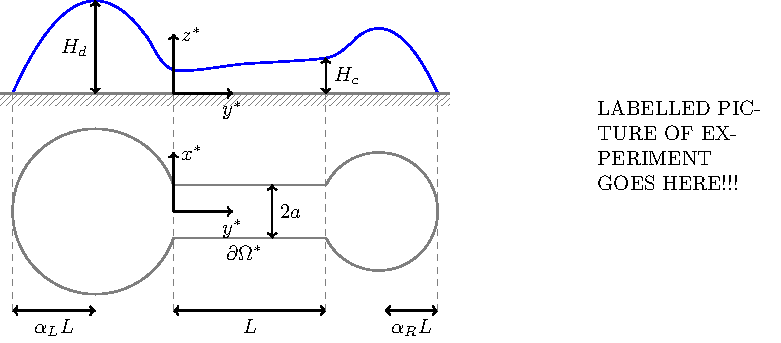
\includegraphics[width=1\linewidth]{Figures/Dumbbell_Dimensional.eps}}  
%   \caption{
%   The geometry and relevant lengths for a simple dumbbell  shaped circuit.
% The side view shows a cross-section of the device on the line of symmetry, ${x^*}=0$, with the origin in middle of the conduit where  it intersects the left drop. 
% The top view shows the contact set of the device bounded by $\partial \Omega^*$ which does  not change over course of an experiment. 
%  The length $L$   is the distance along the outer edge of the  conduit  the width of which is    $ 2a$. 
% The radii of the bases of the two drops are denoted $\alpha_L L$ and $\alpha_R L$; without loss of generality we assume the left drop has the larger base. 
% } \label{fig: geometry}
% \end{figure}
% %%%%%%%%%%%%%%%%%%%%%%%%%%%%%%%%%%%%%%%%%%%%%%%%%%%%%%%%%%%%%%%%%%%%%%%%%
% % This was made in latex using the file Dumbbell_Dimensional.tex  
% %%%%%%%%%%%%%%%%%%%%%%%%%%%%%%%%%%%%%%%%%%%%%%%%%%%%%%%%%%%%%%%%%%%%%%%%%

\subsection{Geometry for a dumbbell shaped circuit}

The simplicity of the new devices means that complex circuits  can be easily and quickly  made by printing multiple  drops and conduits. 
The simplest passive  experimental set-up  is the dumbbell shape contact set shown in figure \ref{fig: geometry}?.  
The circuit is printed under a layer of FC40 of constant  depth $H_{FC40}$ and  consists of a    conduit  of width $2a$ and length $L$, with   fluid drops  of  base radii $R_L=\alpha_L L$ and $R_R=\alpha_R L$  (for the left- and right-hand drops respectively)   at either end.
We assume that the centres of the two drops are such that the length $L$ is the distance along the straight outer edge of the conduit as shown in figure \ref{fig: geometry}f.
Depositing different volumes in each drop,  or using different base radii, then sets up a pressure difference which drives fluid along the conduit.
A flow can then be maintained in the conduit, potentially  for several hours.
We let $H_d$ denote the height scale in a drop and $H_C$ the height scale in the conduit as shown in  figure \ref{fig: geometry}f.
Without loss of generality we will from now on let the left drop have the largest base radius 



\subsection{Governing lubrication equations}

Throughout we shall assume that the fluid contained within the contact line   forms a thin layer so that $\delta = H_d /L \ll1$.
The FC40  is denser than water and so gravity generates a force which acts in the positive ${z^*}$-direction (upwards).
Furthermore,  this is the only effect we need to consider in the thin-film limit; in particular,  the viscosity of the upper fluid does not alter the dynamics at leading order. 
We introduce the Cartesian coordinates $({x^*},{y^*},{z^*})$ and time $t^*$, where the  asterisks    denote variables that are  dimensional.
The  rigid, impermeable substrate is on the  plane  ${z^*}=0$ and   ${y^*}$ is the distance along the  conduit from the intersection with the  left drop as shown in {f}igure \ref{fig: geometry}.
The location of the free surface of the fluid  is denoted by  ${z^*}= {h^*}({x^*},{y^*},{t^*})$ with  the film thickness $h^*$  assumed to be single-valued.
The large advancing and small receding contact angles ensure that   for most experiments the contact line $\partial \Omega^*$ is pinned. 
The components of velocity in the ${x^*}$-, ${y^*}$-  and ${z^*}$-directions are denoted by ${u^*}({x^*},{y^*},{z^*},{t^*})$,  ${v^*}({x^*},{y^*},{z^*},{t^*})$ and   ${w^*}({x^*},{y^*},{z^*},{t^*})$, respectively,   where ${p^*}({x^*},{y^*},{z^*},{t^*})$ denotes the pressure field.
We assume that the pressure in the FC40 is entirely   hydrostatic, so that the the pressure in the FC40 is given by 
\begin{equation}
    p^*_{\text{FC40}} = \rho_2 g \left(H_{\text{FC40}}- z^* \right) +p_{\text{atm}},
\end{equation} 
where $p_{\text{atm}}$ is  atmospheric pressure and $H_{\text{FC40}}$ is the depth of the FC40..
The liquid   in the device  is assumed to be incompressible with constant density $\rho_1$ and   governed by the lubrication 
equations with a constant viscosity $\mu_1$:
\refstepcounter{equation} \label{eqn: thin-film dimensional}
\begin{equation}
\pD{{p^*}}{{x^*}}{}=\mu \pD{{u^*}}{{z^*}}{2}, \quad  \pD{{p^*}}{{y^*}}{}=\mu \pD{{v^*}}{{z^*}}{2} , \quad \pD{{p^*}}{{z^*}}{} = -\rho_1 g , \quad \pD{{u^*}}{{x^*}}{}  +  \pD{{v^*}}{{y^*}}{}  +  \pD{{w^*}}{{z^*}}{} =0. 
\tag{\theequation a--d}
\end{equation}
for $ 0<{z^*}<{h^*}({x^*},{y^*},{t^*})$ and $({x^*}, {y^*}) \in \Omega^*$. 
There is no-slip on the substrate so 
\refstepcounter{equation} \label{eqn: no-slip}
\begin{equation}
{u^*}=0,\quad {v^*}=0,\quad {w^*}=0 \quad \text{on ${z^*}=0$ for ${x^*}, {y^*} \in \Omega^*$.} \tag{\theequation a--c}
\end{equation}
On the fluid interface there is zero shear stress 
\refstepcounter{equation} \label{eqn: interface BC}
\begin{equation} 
\pD{{u^*}}{{z^*}}{}=0, \quad \pD{{v^*}}{{z^*}}{}=0,   \quad {w^*} = \pD{{h^*}}{{t^*}}{}+ {u^*}\pD{{h^*}}{{x^*}}{} + {v^*} \pD{{h^*}}{{y^*}}{} \tag{\theequation a--c}
\end{equation}
on ${z^*}={h^*}({x^*},{y^*},{t^*})$ for ${x^*}, {y^*} \in \Omega^*$. 
The jump in traction on the free surface is assumed to be due to a constant surface tension $\gamma$. 
The pressure difference at the interface $h^*$  is then equal to the curvature as given by the Young-Laplace equation.
Linearising gives  
\begin{equation}
{p^*} = p^*_{\text{FC40}}   - \gamma \nabla^2 {h^*}  \quad \text{on ${z^*}={h^*}({x^*},{y^*},{t^*})$ for ${x^*}, {y^*} \in \Omega^*$. } \label{eqn: laplace dimensional}
\end{equation}
Combining (\ref{eqn: laplace dimensional}) with (\ref{eqn: thin-film dimensional}c)   then shows that the pressure satisfies  
\begin{equation}
{p^*} =  p_{\text{atm}} +\rho_2 g H_{\text{FC40}} - \gamma \nabla^2 {h^*} - \Delta \rho g {h^*}  - \rho_1g   {z^*} ,
\end{equation}   
where $ \Delta \rho = \rho_2-\rho_1$. 
The velocity components are then found from (\ref{eqn: thin-film dimensional}), (\ref{eqn: no-slip}) and (\ref{eqn: interface BC}): 
\refstepcounter{equation}  \label{eqn: velocity dimensional}
\begin{equation}
{u^*} = \frac{1}{2 \mu}\left( {{z^*}}^2  - 2  {h^*} {z^*} \right) \pD{{p^*}}{{x^*}}{}, \quad  {v^*} = \frac{1}{2\mu}\left( {{z^*}}^2  - 2 {h^*} {z^*} \right) \pD{{p^*}}{{y^*}}{} .  \tag{\theequation a,b}
\end{equation}
Finally (\ref{eqn: thin-film dimensional}d), (\ref{eqn: no-slip}c) and (\ref{eqn: interface BC}c) give
\begin{equation}
\pD{{h^*}}{{t^*}}{} = \nabla \cdot \left(\frac{{h^*}^3}{3 \mu } \nabla {p^*} \right)\quad \text{for ${x^*},{y^*} \in \Omega^*$,}  \label{eqn: lubrication dimensional}
\end{equation}
where $\nabla = \left(\partial / \partial x, \, \partial / \partial y  \right)$ is the 2 dimensional gradient operator.
Thus the equation we have to solve for the interface height is given by 
\begin{equation}
 \pD{{h^*}}{{t^*}}{} + \nabla \cdot \left(\frac{1}{3 \mu} {{h^*}}^3 \nabla\left(\gamma \nabla^2 {h^*} + \Delta \rho g {h^*}  \right)\right)=0  \quad \text{for ${x^*},{y^*} \in \Omega^*$.}  \label{eqn: full interface}
\end{equation}
The definitions  and typical values of the  physical parameters  are summarised in table \ref{tab: parameters}. 
 

% The interface height is zero on the contact line and there is no flux through the contact line  so we impose
% \begin{equation}
% {h^*} =0, \quad \pD{{p^*}}{n}{} =0 \note{ or whatever} \label{eqn: contact line dimensional}
% \end{equation}
% on $\partial \Omega$. 
% Finally an initial condition needs to be prescribed for the   interface height at ${t^*}=0$.  










% The velocity, pressure and  interface height are   then assumed to  satisfy the usual lubrication equations, given the thin-film approximation (as we shall describe shortly following the nondimensionalisation).



% The interface height, pressure and velocity  then satisfy the lubrication equations given by 

% eg \cite{Oron1997Long-scaleFilms}??






\subsection{Nondimensionalisation and thin-film reduction}

The drop height and  conduit  length are the natural length scales with which  to non-dimensionalise.
We anticipate that there will be multiple time scales on which different physical effects will be dominant, but we initially use  the time scale of capillary action in the drops.
Thus, we  non-dimensionalise by scaling
\begin{equation*}\label{eqn: scalings 1}
\begin{gathered}
{x^*} = L x,\quad {y^*} = L y, \quad {z^*}=H_d z, \quad  {t^*}=\frac{3 \mu L}{ \delta^3 \gamma } {t},
% \\ {u^*}=\frac{\delta^3 \gamma}{\mu}u, \quad {v^*}=\frac{\delta^3 \gamma}{\mu}v, \quad {w^*}=\frac{\delta^4 \gamma}{\mu}w,
 \\ {h^*} =H_d h
,  \quad {p^*} = \frac{\gamma}{\delta L}  p  +p_{\text{atm}} + \rho_2 gH_{\text{FC40}} - \rho_1 g H_d z  .
\end{gathered}
\end{equation*}
% Here  $p_{\text{atm}}$ is atmospheric pressure, while $\rho_2$,  $H_{\text{FC40}}$ are respectively the density and depth of the FC40.
We let $\Omega $ denote the rescaled contact set bounded by  the pinned contact line $\partial \Omega$. 
The governing equation for the interface height (\ref{eqn: full interface}) is then given by
\refstepcounter{equation} \label{eqn: lubrication} 
\begin{equation}
\pD{h}{{t}}{} =   \nabla \cdot \left( h^3 \nabla p \right), \quad p=-\nabla^2 h  - {Bo}\,h   \quad \text{for $ (x,y) \in \Omega $} , \tag{\theequation a,b}
\end{equation}
 where the Bond number is defined as ${Bo} =  \left(\rho_2 -\rho_1  \right)g L^2 / \gamma $. 
The interface height is zero on the contact line and there is no flux through the contact line,   so we impose the boundary  conditions
\refstepcounter{equation}\label{eqn: contact line}% Correctly mark and label
\begin{equation}
h = 0,  \quad h^3 \pD{p}{n}{} =0 \quad   \text{ for }(x,y) \in \partial \Omega , \tag{\theequation a,b} 
\end{equation} 
where $\partial / \partial n$  denotes the outward normal derivative on $ \partial \Omega$; we note that   a local analysis at the contact line reveals that instead of (\ref{eqn: contact line}b) it would be sufficient to impose a finite contact angle at the contact line ({\it{i.e.}}\ $\partial h/ \partial n = O(1)$ on $\partial \Omega$)  as in \cite{Lacey1982TheSurface}.
Finally an initial condition needs to be prescribed for the   interface height at time $t=0$.  
\begin{equation}
    h(x,y,0) = \mathcal{H}(x,y) \quad \text{for $ (x,y) \in \Omega $.}  \label{eqn: initial}
\end{equation}
 The   model (\ref{eqn: lubrication})--(\ref{eqn: initial}) depends on    five  dimensionless parameters.  
 The parameter  $\delta = H_d/L$  is the ratio of the vertical and horizontal length scales of the circuit.
 The aspect ratio of the  conduit  $\epsilon = a/L $  gives a ratio of the  conduit  width to length.
The Bond number $Bo$  gives a  measure of the importance of gravitational forces compared to surface tension.
The dimensionless radii of the bases of the two drops are denoted by $\alpha_L$ and $\alpha_R$.







% We let $\Omega $ denote the rescaled contact set bounded by  the pinned contact line $\partial \Omega$. 
% Since the velocity in the $z^* $ direction is negligible at leading order we find that the  pressure is independent of $z$.
% Then a  balance of momentum across the interface leads to the  linearised Young-Laplace equation for the pressure field, $p(x,y,t)$, given by 
% \begin{equation}
% p = -     \nabla^2 h - {Bo}\, h   \quad  \text{for  $(x,y) \in \Omega$,} \label{eqn: laplace}
% \end{equation} 
%   where the Bond number is defined as ${Bo} =  \left(\rho_2 -\rho_1  \right)g L^2 / \gamma $. 
% At leading order the $x$- and $y$- lubrication equations, the  no-slip and no shear stress conditions    on $z=0$ and  on the interface $z=h$, respectively,  give the velocity   in the $x$- and $y$-directions as 
% \begin{equation}
%     (u,v) =  -z\left( h-\frac{z}{2}  \right)\nabla p  \quad  \text{for $ 0 < z < h(x,y,t)$, $(x,y) \in \Omega$.}
%     \label{eqn: velocity}
% \end{equation}
% % In (\ref{eqn: velocity}) and   everything that follows $\nabla $ denotes the two dimensional operator
% % \begin{equation}
% %     \nabla = \left(\pD{}{x}{}, \pD{}{y}{}\right).
% % \end{equation} 
% %  and similarly for $ \nabla^2$.  
%   The incompressibility condition, the no-flux condition on the substrate   and the kinematic condition on the interface    then give us  the familiar dimensionless Reynolds lubrication  equation    governing the interface height:
% \begin{equation}
% \pD{h}{{t}}{} = \nabla \cdot \left( h^3 \nabla p \right)   \quad \text{for $ (x,y) \in \Omega $} ,  \label{eqn: lubrication}
% \end{equation}
%  where $p$ is given by (\ref{eqn: laplace}).
% The interface height is zero on the contact line and there is no flux through the contact line,   so we impose the boundary  conditions
% \refstepcounter{equation}\label{eqn: contact line}% Correctly mark and label
% \begin{equation}
% h = 0,  \quad h^3 \pD{p}{n}{} =0 \quad   \text{ for }(x,y) \in \partial \Omega , \tag{\theequation a,b} 
% \end{equation} 
% where $\partial / \partial n$  denotes the outward normal derivative on $ \partial \Omega$; we note that   a local analysis at the contact line reveals that instead of (\ref{eqn: contact line}b) it would be sufficient to impose a finite contact angle at the contact line ({\it {i.e.}\ignorespaces} $\partial h/ \partial n = O(1)$ on $\partial \Omega$)  as in \cite{Lacey1982TheSurface}.
% Finally an initial condition needs to be prescribed for the   interface height at time $t=0$.  
% This will be determined by how much fluid is initially printed into  the  conduit  and each drop.
 
%% TABLE %%%%%%%%%%%%%%%%%%%%%%%%
\begin{table}
\centering
\begin{tabular}{l l c l} 
\textbf{Symbol} & \textbf{Definition} &  \textbf{Typical values}    & \textbf{Units}
\\ \hline
$\mu_1$ & Dynamic viscosity (water) & $ \SI{1e-3}{}$  & $ \SI{}{\kilogram\per\meter\per\second}$ 
\\ $\mu_2$ & Dynamic viscosity (FC40) & $ \SI{4.05e-3}{}$  & $ \SI{}{\kilogram\per\meter\per\second}$ 
\\  $\gamma$ & Surface tension (water/FC40) & $\SI{4e-2}{}$  & $\SI{}{\kilogram\per\second\squared}$  
\\    $\rho_1$ & Density  (water)  & $ \SI{1e3}{}$ & $ \SI{}{\kilogram\per\meter\cubed}$ 
\\   $\rho_2$ & Density   (FC40)  & 
$ \SI{1.85e3}{}$  & 
$ \SI{}{\kilogram\per\meter\cubed}$ 
\\ $g$ & Gravity  & $ \SI{9.81}{}$ & $ \SI{}{\meter\per\second\squared}$
\\ $H_{FC40}$ & Depth of the FC40  & $  3$  & $ \SI{}{\milli\meter}$
\\ $H_d$ & Maximum height of drop  & $ < 3$  & $ \SI{}{\milli\meter}$
\\ $L$ &  Conduit  length  & $ \SIrange{1.5}{30}{}$ & $ \SI{}{\milli\meter}$ 
\\ $a$ & Half  conduit  width  & $ \SIrange{0.15}{0.75}{}$  & $ \SI{}{\milli\meter}$
% \\ $\alpha_L L,\alpha_R L $ & Base radii of left and right drops  & $ \SIrange{1}{4}{}$   & $ \SI{}{\milli\meter}$ 
\\ $R_L,R_R $ & Base radii of left and right drops  & $ \SIrange{1}{4}{}$   & $ \SI{}{\milli\meter}$ 
\\ $v_L, v_R$ & Volume of fluid in left and right drops & $ \SIrange{2}{20}{}$ & $ \SI{}{\micro\litre}$ 
\\ \hline
 $\delta$ &   $H_d/L$ \quad   & $ < 0.6$   & ---
\\ $\epsilon$ & $a/L$ & $ \SIrange{0.005}{0.5}{}$   & ---
\\ $Bo $ & $(\rho_2 -\rho_1 )g L^2/\gamma$ & $ \SIrange{0.5}{188}{}$  & ---
\\ $\alpha_{L,R}$   &   $R_{L,R}/{L} $   & $ \SIrange{0.03}{2.7}{}  $ & ---
\\ \hline
 \end{tabular}
\caption{The   physical parameters for water and FC40 at room temperature and pressure, the typical range of geometric parameters  used and the dimensionless parameters. 
Unless stated otherwise the physical parameters (for water and FC40 and gravity)  are used throughout. 
Throughout we assume that $\delta \ll 1$, and $\alpha_L \geq \alpha_R$.
All dimensional values are  from  \cite{Walsh2017MicrofluidicsWalls}.  
}
\label{tab: parameters}
\end{table} 
%%%%%%%%%%%%%%%%%%%%%%%%%%%%%%%%%%%%%%%%%%%%%%%%%%%%%%%%%%%


 

% \begin{equation}
% \pD{{p^*}}{{x^*}}{}=\mu \pD{{u^*}}{{z^*}}{2}, \quad  \pD{{p^*}}{{y^*}}{}=\mu \pD{{v^*}}{{z^*}}{2} , \quad \pD{{p^*}}{{z^*}}{} = -\rho_1 g , \quad \pD{{u^*}}{{x^*}}{}  +  \pD{{v^*}}{{y^*}}{}  +  \pD{{w^*}}{{z^*}}{} =0 \label{eqn: thin-film dimensional}
% \end{equation}
% for $ 0<{z^*}<{h^*}({x^*},{y^*},{t^*})$ and ${x^*}, {y^*} \in \Omega$. 
% There is no-slip on the substrate so 
% \begin{equation}
% {u^*}=0,\quad {v^*}=0,\quad {w^*}=0 \label{eqn: no-slip}
% \end{equation}
% on ${z^*}=0$ for ${x^*}, {y^*} \in \Omega$. 
% On the fluid interface there is zero shear stress 
% \begin{equation}
% \pD{{u^*}}{{z^*}}{}=0, \quad \pD{{v^*}}{{z^*}}{}=0,   \quad {w^*} = \pD{{h^*}}{{t^*}}{}+ {u^*}\pD{{h^*}}{{x^*}}{} + {v^*} \pD{{h^*}}{{y^*}}{} \label{eqn: interface BC}
% \end{equation}
% on ${z^*}={h^*}({x^*},{y^*},{t^*})$ for ${x^*}, {y^*} \in \Omega$. 

% % eg \cite{Oron1997Long-scaleFilms}??
% The velocity components are then found from (\ref{eqn: thin-film dimensional}), (\ref{eqn: no-slip}) and (\ref{eqn: interface BC}): 
% \begin{equation}
% {u^*} = \frac{1}{2 \mu}\left( {{z^*}}^2  - 2  {h^*} {z^*} \right) \pD{{p^*}}{{x^*}}{}, \quad  {v^*} = \frac{1}{2\mu}\left( {{z^*}}^2  - 2 {h^*} {z^*} \right) \pD{{p^*}}{{y^*}}{} . \label{eqn: velocity dimensional}
% \end{equation}
% The pressure then satisfies
% \begin{equation}
% {p^*} =  p_{\text{atm}} +\rho_2 g H - \gamma \nabla^2 {h^*} - \Delta \rho g {h^*}  + \rho_1g   {z^*} ,
% \end{equation}   
% where $ \Delta \rho = \rho_2-\rho_1$.
% Finally (\ref{eqn: thin-film dimensional}d), (\ref{eqn: no-slip}c) and (\ref{eqn: interface BC}c) give

% Thus the equation we have to solve for the interface height is given by 
% \begin{equation}
%  \pD{{h^*}}{{t^*}}{} + \nabla \cdot \left(\frac{1}{3 \mu} {{h^*}}^3 \nabla\left(\gamma \nabla^2 {h^*} + \Delta \rho g {h^*}  \right)\right)=0 \label{eqn: full interface}
% \end{equation}
% for ${x^*},{y^*} \in \Omega$.



% We  non-dimensionalise with 
% \begin{equation}
% \bm{x} = L \bm{x}, \quad h=H_d h  , \quad 
%  t=\frac{3 \mu L}{ \delta^3 \gamma } t. do p also!!
% \end{equation}
% and Bond  and delta 

% \begin{equation}
%  \pD{h}{t}{} + \nabla \cdot \left(  {h}^3 \nabla\left(  \nabla^2 h + Bo\, h  \right)\right)=0 \label{eqn: lubrication nondim}
% \end{equation}
% for $x,y \in \Omega$.





% %   \subsection{Dimensionless parameters}

% %% TABLE %%%%%%%%%%%%%%%%%%%%%%%%
% \begin{table}
% \centering
% \begin{tabular}{l l l} 
% \textbf{Symbol} & \textbf{Definition} &  \textbf{Typical ranges}  \vspace{4px}
% \\ $\delta$ &  \multicolumn{1}{c}{ \(\displaystyle \frac{H_d}{L}\)}    & $ < 0.6$   
%  \vspace{4px}
% \\ $\epsilon$ & \multicolumn{1}{c}{  \(\displaystyle \frac{a}{L}\) } & $ \SIrange{0.005}{0.5}{}$    \vspace{4px}
% \\ $Bo $ & \multicolumn{1}{c}{ \(\displaystyle \frac{\left(\rho_2 -\rho_1  \right)g L^2}{ \gamma} \) } & $ \SIrange{0.5}{188}{}  $\vspace{4px}
% \\ $\alpha_{L,R}$   &  \multicolumn{1}{c}{  \(\displaystyle \frac{R_{L,R}}{L} \)}   & $ \SIrange{0.03}{2.7}{}  $   \vspace{4px}
%  \end{tabular}
% \caption{The dimensionless parameters and their typical ranges as estimated from the values in {t}able \ref{tab: parameters}. 
% Throughout we assume that $\delta \ll 1$, and $\alpha_L \geq \alpha_R$.
% % Find actual laregst and smallest of these from paper, big won't go with small l
% }
% \label{tab: nondim parameters}
% \end{table} 
% %%%%%%%%%%%%%%%%%%%%%%%%%%%%%%%%%%%%%%%%%%%%%%%%%%%%%%%%%%%



% \subsubsection{\note{Possible alternative scaling}}
% \note{Let $ \delta = v^*/R^3$, where $v^*$ and $R$ are the volume and base radius of the tallest drop respectively. 
% Then $H_d \sim v^*/R^2$, everything that follows is the same except that $\delta $ can be written in terms of things that are easier to measure.}




\subsection{Global mass conservation consideration}
 
One of our main aims will be to predict the time scale  over which  the volumes of the two drops  equilibrate; {\it {i.e.}\ignorespaces}  the time scale of   drop drainage. 
We divide the contact set $\Omega$ into 3 regions, the conduit region  is defined by $\Omega_C=\{ (x,y)  : \ 0<y <1, \ |x| <\epsilon   \}$,  then the   left-hand drop region is bounded by  circular arc of radius $\alpha_L$ which intersects the conduit at $(x,y) = (\pm \epsilon,  0 )$, the right-hand drop region is similarly defined as shown in figure \ref{fig: geometry, dimensionless}. 
We define the leading-order volumes in the left drop,  conduit  and right drop to be  given by  
\refstepcounter{equation}\label{eqn: vols}
\begin{equation}
{V_L}({t}) = \iint\limits_{\Omega_L} {h} \dv{{x}}\! \dv{{y}} ,\quad {V_C}({t}) = \iint\limits_{\Omega_C} {h} \dv{{x}}\! \dv{{y}} ,\quad {V_R}({t}) = \iint\limits_{\Omega_R} {h} \dv{{x}}\! \dv{{y}}, \tag{\theequation a--c} 
\end{equation}   
Since  there is no flux of liquid through the pinned contact line,  the total volume in the device is given by the initial volume, $V$  say, as follows 
\begin{equation}
{V_L} +{V_C}+{V_R}  = \iint\limits_{\Omega} {h} ({x},{y},0)\dv{{x}}\! \dv{{y}} ={V}. 
\end{equation}
The dimensionless area of, and flux through, a  cross-section  of the conduit in a   ${y}$-plane (with $0<{y}<1$) are given at leading order by  
\refstepcounter{equation}\label{eqn:  conduit  flux area} % Correctly mark and label
\begin{equation}
{A}({y},{t}) = \int_{-\epsilon}^{\epsilon} {h} \dv{{x}}, \quad {Q}({y},{t}) =\int_{-\epsilon}^{\epsilon} \int_0^{h} {v}\dv{{z}}\! \dv{{x}} = -\int_{-\epsilon}^{\epsilon} {h}^3 \pD{{p}}{{y}}{} \dv{{x}} .  \tag{\theequation a,b} 
\end{equation} 
% \begin{equation}
% {A}({y},{t}) = \int_{-\epsilon}^{\epsilon} {h} \dv{{x}}, \quad {Q}({y},{t}) =\int_{-\epsilon}^{\epsilon} \int_0^{h} {v}\dv{{x}}\! \dv{{z}} = -\int_{-\epsilon}^{\epsilon} {h}^3 \pD{{p}}{{y}}{} \dv{{x}} .  \label{eqn:  conduit  flux area}
% \end{equation}  
Integrating  (\ref{eqn: lubrication}) over the  conduit  cross-section  then gives 
\begin{equation}
\pD{{A}}{{t}}{} + \pD{{Q}}{{y}}{}=0\quad \text{for $0<{y}<1$.} \label{eqn: mass conserve dim 1}
\end{equation}
Alternatively,  integrating (\ref{eqn: lubrication})   over the three regions $\Omega_L$, $\Omega_C$ and $\Omega_R$ shows how the volume is changing in each region over time according to the relations
\refstepcounter{equation} \label{eqn: flux odes}  % Correctly mark and label
\begin{equation}
\D{{V_L}}{{t}}{}  = -{Q_L}({t}), 
\quad  \D{{V_R}}{{t}}{} =   {Q_R}({t}),
\quad  \D{{V_C}}{{t}}{}  = {Q_L}({t})-{Q_R}({t}), \tag{\theequation a--c} 
\end{equation} 
% \begin{equation}
% \D{{V_L}}{{t}}{}  = -{Q_L}({t}), 
% \quad  \D{{V_R}}{{t}}{} =   {Q_R}({t}),
% \quad  \D{{V_C}}{{t}}{}  = {Q_L}({t})-{Q_R}({t}), \label{eqn: flux odes}
% \end{equation}
where we have defined $Q_L(t) =  Q(0,t)$ and $Q_R(t) =  Q(1,t)$ to be the fluxes where the  conduit  connects to the left and right drop respectively.
The   expressions (\ref{eqn: mass conserve dim 1})  and (\ref{eqn: flux odes})     will play a key role in our scaling and subsequent asymptotic analysis, in which they will be used to close the leading-order governing equations (rather than proceeding to higher order).

%%%%%%%%%%%%%%%%%%%%%%%%%%%%%%%%%%%%%%%% FIGURE %%%%%%%%%%%%%%%%%%%%%%
\begin{figure} 
\centering
 {\includegraphics[width=0.8\linewidth]{Figures/Dumbbell_Dimensionless.eps}}  
  \caption{ 
  The dimensionless contact set with each of the  domains labelled; $\Omega_C$ is the conduit, a rectangle of length 1 and width $2 \epsilon$; $\Omega_{L,R}$ are bases of the drops; $\Omega_{JL,R}$ are the junction regions where the drops intersect the conduit and $\partial \Omega$ is the pinned contact line. 
} \label{fig: geometry, dimensionless}
\end{figure}
%%%%%%%%%%%%%%%%%%%%%%%%%%%%%%%%%%%%%%%%%%%%%%%%%%%%%%%%%%%%%%%%%%%%%%%%%
% This was made in latex using the file Dumbbell_Dimensionless.tex  
%%%%%%%%%%%%%%%%%%%%%%%%%%%%%%%%%%%%%%%%%%%%%%%%%%%%%%%%%%%%%%%%%%%%%%%%%


 
%     _______. _______   ______ .___________. __    ______   .__   __. 
%    /       ||   ____| /      ||           ||  |  /  __  \  |  \ |  | 
%   |   (----`|  |__   |  ,----'`---|  |----`|  | |  |  |  | |   \|  | 
%    \   \    |   __|  |  |         |  |     |  | |  |  |  | |  . `  | 
%.----)   |   |  |____ |  `----.    |  |     |  | |  `--'  | |  |\   | 
%|_______/    |_______| \______|    |__|     |__|  \______/  |__| \__/
\section{Asymptotic  analysis for a long, thin conduit  } \label{sec: times}

 \subsection{Asymptotic structure and time scales } \label{sec: time scales}

 
 
The two main aims of the dumbbell  set-up are 
(i) for the pressure difference between the two  drops to be the dominant mechanism that drives fluid through the conduit; and 
(ii) for the flux through the  conduit  to be slowly varying over the time scale of hours, as relevant for  experiments.
The first aim requires the pressure in the drops and  conduit  to be comparable,  while the second requires the  conduit  to be much thinner and narrower than the drops, {\it {i.e.}\ignorespaces} a rivulet. 
We focus  henceforth on the distinguished limit in which $Bo,\alpha_L,\alpha_R = O(1)$, we further suppose that the drops may be  large enough that we must account for the effects of gravity,  but not so large that gravity dominates the effects of  surface tension.
To achieve aim (i) we  require the pressure in the drops and conduit to be comparable.
In the conduit we   scale $ x \sim \epsilon$,   balancing  the pressure   with the first term on the right-hand side of  (\ref{eqn: lubrication}b) shows that we must print liquid of thickness  $ h \sim \epsilon^2 $ in the conduit.
To achieve aim (ii) we require the conduit to be long and narrow  {\it {i.e.}\ignorespaces}  $ \epsilon  = a/L \ll 1$.
Thus,  the  asymptotic  structure consists  of  five regions: two drops   with contact sets $\Omega_L$ and $\Omega_R$, a narrow and thin conduit with contact set $\Omega_C$, and two small junction regions with contact sets $\Omega_{JL}$ and $\Omega_{JR}$  connecting together the drops and conduit  as illustrated in  {f}igure  \ref{fig: geometry, dimensionless}. 
The typical ranges of the dimensionless parameters are shown in {t}able \ref{tab: parameters}.
Both $\epsilon$ and $\delta$ do not exceed unity.
%  But as the height of the drop becomes comparable to the depth of the FC40 we  expect the thin-film  model  to perform poorly and the case $\delta =O(1)$ will be considered elsewhere.

  
 
Given our assumptions about the geometry of the device  we can now describe the different physical  time scales and show that drainage (the time scale on which the pressure equilibrates) acts on a  much  longer time scale than anything else in the model.
 In the three regions we have defined  we can use a dominant balance argument in (\ref{eqn: lubrication}) to  find  the time scale of capillary action in each region. 
In  the  conduit  region we scale with     $x \sim\epsilon$ and $h \sim \epsilon^2$;  in the junction region we scale with   $x,y,h \sim \epsilon$.
These scalings and (\ref{eqn: lubrication}) give  us the dimensionless  time scales of capillary action in the junction  and  conduit, respectively, as $t_J\sim \epsilon$  and $t_{CW}\sim\epsilon^{-2}  $.  
Since we  assume that the  conduit  is much longer than it is wide $t_{CW}$ is the time scale of relaxation  (of the free boundary) across the width of the conduit.
The time scale of relaxation of the free boundary along the length of the conduit is found by balancing the terms in (\ref{eqn: mass conserve dim 1}).
The cross-sectional area and flux are only defined in the conduit so  (\ref{eqn:  conduit  flux area}) are also  rescaled with  $x \sim\epsilon$ and  $h \sim \epsilon^2$,  so that  $A \sim \epsilon^4$  and $Q \sim \epsilon^7$; hence    the time scale for relaxation along the length of the conduit is $t_{CL} \sim \epsilon^{-4}  $. 
The drainage time scale is then found by balancing the terms in  (\ref{eqn: flux odes}).
With  the same length scales as above for the flux,  we still  have $Q \sim \epsilon^7$, but the relevant length scale for the volume gives $ V_L =O(1)$ (since all the fluid is contained in the drop regions at leading order).
Thus the time scale for drop drainage is $ t_{DD} \sim \epsilon^{-7}$.


We have identified five time scales in this section each depending on the conduit aspect ratio $\epsilon$. 
They are, respectively,  the relaxation time scales for the junction,  drops,  conduit width and  conduit length and the drainage time scale:
\refstepcounter{equation}  \label{eqn: time scales} 
 \begin{equation}
t_{J} \sim \epsilon  , \quad  t_{D} \sim 1, \quad    t_{CW}\sim \frac{1}{\epsilon^2}, \quad  t_{CL} \sim \frac{1}{\epsilon^4}  , \quad t_{DD}\sim \frac{1}{\epsilon^7}.  \tag{\theequation a--e}
 \end{equation}
To achieve slowly varying fluxes and stresses we need to be on a time scale much longer than $t_{CL}$, and  we can also  already see that the drainage time scale is very sensitive to $\epsilon$, so that the geometry is the a very  important factor in achieving a quasi-steady flux.




%     _______. _______   ______ .___________. __    ______   .__   __. 
%    /       ||   ____| /      ||           ||  |  /  __  \  |  \ |  | 
%   |   (----`|  |__   |  ,----'`---|  |----`|  | |  |  |  | |   \|  | 
%    \   \    |   __|  |  |         |  |     |  | |  |  |  | |  . `  | 
%.----)   |   |  |____ |  `----.    |  |     |  | |  `--'  | |  |\   | 
%|_______/    |_______| \______|    |__|     |__|  \______/  |__| \__/
% \section{Solutions in the drops,  conduit  and junctions}
\subsection{Quasi-steady solution in the drops}\label{sec: drops}
At leading order   the relevant contact set in each drop is a circular disc since the  conduit  is in the much smaller junction region.
For $t \gg t_{D} \sim 1$,   the profile in each  drop region will be quasi-steady and axisymmetric, with spatially uniform pressure at leading order.  
The leading order analysis is the same in each drop, so we give only the details for the left-hand one.
We introduce  the  polar coordinate $r=\sqrt{x^2 +y^2}$   measuring   radial distance   from the centre of the circular contact set of the  left-hand drop.  
Then, expanding $h \sim h_L(r,t)$  and $ p\sim p_L(t)$ as $\epsilon \to 0$, (\ref{eqn: lubrication}b) gives the familiar  leading-order governing equation  for the height in the  left-hand drop given by
\begin{equation}
\pD{h_L}{r}{2}  +\frac{1}{r} \pD{h_L}{r}{} +Bo\, h_L = -p_L  \quad \text{for $  0<r<\alpha_L$.}  \label{eqn: bessel}
\end{equation}
Since the contact set  is a circle of radius $\alpha_L $ at leading order, we impose the boundary condition   $h_L(\alpha_L ,t)=0$; we   expect the solution to be bounded at the origin, so we also  require that $h_L(0,t) < \infty$.
The pressure is fixed by imposing the volume of fluid in the drop so that 
\begin{equation}
 2 \pi \int_0^{\alpha_L} r \, h_L\dv{r} = V_L(t).
\end{equation}  
The solution which satisfies these  conditions is given by 
\refstepcounter{equation}\label{eqn: drop height left}% Correctly mark and label
\begin{equation}
 h_L=\left(  \frac{     \besselj{0}{\sqrt{Bo}\, r }  }{ \besselj{0}{\sqrt{Bo} \,\alpha_L }  } -1  \right) \frac{p_L}{Bo}, \quad  p_L = \frac{ Bo \, \besselj{0}{\Phi_L}}{\pi \alpha_L^2 \besselj{2}{\Phi_L } }V_L
,  \tag{\theequation a,b} 
\end{equation}
where $ J_n$  is the Bessel function of the first kind of order $n$ and 
  $\Phi_L = \alpha_L\sqrt{Bo}  $.
Similarly in the right-hand drop we obtain
\refstepcounter{equation}\label{eqn: drop height right}% Correctly mark and label
\begin{equation}
 h_R=\left(  \frac{     \besselj{0}{\sqrt{Bo}\, r}}{ \besselj{0}{\sqrt{Bo} \,\alpha_R}} -1  \right) \frac{p_R}{Bo}, \quad   p_R = \frac{Bo  \, \besselj{0}{\Phi_R }}{\pi \alpha_R^2 \besselj{2}{\Phi_R}}V_R, \tag{\theequation a,b}  
  \end{equation}
  where $\Phi_R =\alpha_R \sqrt{Bo}  $.
 
 
 
\subsection{Quasi-steady solution in the conduit}


% %%%%%%%%%%%%%%%%%%%%%%%%%%%%%%%%%%%%%%%% FIGURE %%%%%%%%%%%%%%%%%%%%%%
% \begin{figure} 
% \centering
%  {\includegraphics[width=1\linewidth]{Figures/Paper_1_Junction_Problem_Figure.pdf}}  
%   \caption{ 
%   The leading- and second-order problems in the junction region.
% (a) At leading-order the height is zero on the contact line and also tends to zero in the conduit as $\bar{y} \to 0$ since the interface height is $O(\epsilon)$ there.
% The drop occupies the lower part of the $\bar{z}$-plane, expanding the solution in  the drop  (\ref{eqn: drop height left}) for $r \sim \epsilon$ as $\epsilon \to 0$ gives the leading-order far-field condition as  $ \bar{x}^2+ \bar{y}^2 \to \infty$. 
% (b) At second-order the interface height is still zero on the contact line in the conduit, but on $ \bar{y}$ we have to take account of the curvature of the contact line.
% In the conduit the far-field condition comes from matching with the conduit solution (\ref{eqn:  conduit  height}), in the drop the far-field condition is the $O(\epsilon)$ term in the expansion of  (\ref{eqn: drop height left}) with  $r \sim \epsilon$.
% } \label{fig: junction geometry}
% \end{figure}
% %%%%%%%%%%%%%%%%%%%%%%%%%%%%%%%%%%%%%%%%%%%%%%%%%%%%%%%%%%%%%%%%%%%%%%%%%
% % This was made in latex using the tikz package in the Overleaf project Paper 1 Junction Problem Figure
% %%%%%%%%%%%%%%%%%%%%%%%%%%%%%%%%%%%%%%%%%%%%%%%%%%%%%%%%%%%%%%%%%%%%%%%%%










The footprint of the  conduit  is   a rectangle of  width $2\epsilon$ and length $1$.
On the long edges of the  conduit  the interface will have zero height where the contact line is pinned.
The appropriate boundary condition on the short edge will be derived below by matching with the junction region.
Earlier we deduced that we need $h\sim \epsilon^2 $ in order for the pressure difference between the drops to be the dominant  mechanism driving the flow.
Thus we  rescale the governing equations with  
\begin{equation*}
{x} = \epsilon \, \widehat{x},  \quad h= \epsilon^2 \,\widehat{h}_C.   
\end{equation*}
Provided $t \gg t_{CW}\sim \epsilon^{-2}$, the pressure is spatially uniform in each ${y}$-plane at leading order. Expanding $\widehat{h}\sim \widehat{h}_C(\widehat{x},y,t)$ and $ p\sim p_C(y,t)$ as $ \epsilon \to 0$ in  (\ref{eqn: lubrication}b) then gives
\begin{equation}
 \pD{\widehat{h}_C}{\widehat{x}}{2}=- p_C \quad \text{for $ -1 < \widehat{x}<1$.} \label{eqn: leading channel}
\end{equation} 
Since $\widehat{h}_C = 0$ at $ \widehat{x} = \pm1$  for $0 < y < 1$, we deduce that the interface height has a parabolic profile in  each cross-section given by  
\begin{equation}
\widehat{h}_C = \frac{p_C}{2} \left( 1-\widehat{x}^2  \right) . \label{eqn:  conduit  height}
\end{equation}
As is shown in table \ref{tab: parameters} there may be regimes for which $ \epsilon^2 Bo  $ is not small.   
In this case the leading order solution in the cross-section can   be found in terms of a  cosine function, this would  not alter the arguments that follow,  although the composite solution would then be much harder to compute.
It follows from (\ref{eqn:  conduit  flux area}) that the corresponding leading order expressions for the area and flux in the conduit  are given by
\refstepcounter{equation}\label{eqn: area and flux}  
\begin{equation}
A \sim \frac{2}{3}\epsilon^3 p_C, \quad 
Q \sim -\frac{1}{35}  \epsilon^7  \pD{}{{y}}{}\left( p_C^4 \right) \quad \text{as $\epsilon \to 0$.}   \tag{\theequation a,b} 
\end{equation} 
% \begin{equation}
% A \sim \frac{2}{3}\epsilon^3 p_C, \quad 
% Q \sim -\frac{1}{35}  \epsilon^7  \pD{}{{y}}{}\left( p_C^4 \right).  \label{eqn: area and flux}
% \end{equation}
A clear picture of what is happening  in the junction regions is needed before proceeding with the leading order solution for the pressure. 









\subsection{Quasi-steady solution in  the junction regions}  \label{sec: junction}

The junction   regions connecting the  conduit  to the drops are  indicated by the   boxes in figure \ref{fig: geometry, dimensionless}.
 Without loss of generality we will consider only the junction connecting the  conduit  to the left drop.
 Since the film thickness is of   $ O(1) $ in the drop   the pertinent scalings in the left-hand  junction region  are given by  
\begin{equation*}
 x = \epsilon \widebar{x}, \quad y = \epsilon   \widebar{y} , \quad h=\epsilon   \widebar{h}.  \label{eqn: junction scaling}
\end{equation*}  
 The contact  line of the left-hand drop then satisfies
\begin{equation}
 \epsilon^2 \widebar{x}^2 + \left( \epsilon \widebar{y} +\sqrt{\alpha_L^2-\epsilon^2} \right)^2 = \alpha_L^2  \quad \text{for $\widebar{y} \leq0$,} \label{eqn: expanded footprint} 
\end{equation} 
so that it lies at $ \widebar{y} =0$ for $ | \widebar{x}| \geq 1$ at leading order as $\epsilon \to 0$.
%%%%%%%%%%%%%%%%%%%%%%%%%%%%%%%%%%%%%%%% FIGURE %%%%%%%%%%%%%%%%%%%%%%
\begin{figure} 
\centering
 {\includegraphics[width=1\linewidth]{Figures/Junction_Problem.eps}}  
  \caption{ 
 (a) The leading- and (b) the second-order problems in the junction region, where $ \Omega_J =\{ (\bar{x},\bar{y})  : \ \bar{y} <0 \} \cup \{ (\bar{x},\bar{y})  : \ |\bar{x} | <1 \bar{y} \geq0 \}$, see text for details.
} \label{fig: junction geometry}
\end{figure}
%%%%%%%%%%%%%%%%%%%%%%%%%%%%%%%%%%%%%%%%%%%%%%%%%%%%%%%%%%%%%%%%%%%%%%%%%
% This was made in latex using the file Junction_Problem.tex  
%%%%%%%%%%%%%%%%%%%%%%%%%%%%%%%%%%%%%%%%%%%%%%%%%%%%%%%%%%%%%%%%%%%%%%%%%
The leading-order geometry of the contact set in the junction region is therefore as  illustrated in   {f}igure \ref{fig: junction geometry}: the contact set of the  drop fills the lower half-plane $\widebar{y} < 0$, while that of    the    conduit  fills the semi-infinite strip $|\widebar{x}|<1$, $ \widebar{y}\geq0$.
The interface height in the junction region is governed by (\ref{eqn: lubrication}), with   the solution needing to match with   the conduit solution (\ref{eqn:  conduit  height}) as $\widebar{y} \to \infty$ and with  the drop solution (\ref{eqn: drop height left}) as $\widebar{x}^2+\widebar{y}^2 \to \infty $ in the lower half-plane, with  (\ref{eqn: contact line}) still holding on  the contact line.
Therefore,      we need to match the $O(1)$ height in the drops with the $O(\epsilon^2)$ height in the conduit.
But this implies a pressure scaling of $ p  \sim 1/\epsilon   $; a   larger pressure  than  in the drop and conduit.
Thus, the  mean curvature at leading order must be of $ O(1/\epsilon)$ for matching.
For $t \gg t_J\sim \epsilon $  the evolution will be quasi-steady and, as we shall soon see, the pressure will be  spatially uniform.   
Matching the film thickness of the drop and  the  conduit  will require us to proceed  to second  order, so we expand  $\widebar{h} \sim \widebar{h}_0(\widebar{x},\widebar{y}) + \epsilon \widebar{h}_1(\widebar{x},\widebar{y})  $  and $ p\sim p_{JL}$ as $\epsilon \to 0$.
The leading- and second-order problems are summarised in figure \ref{fig: junction geometry}.
At leading-order the height is zero on the contact line (given by (\ref{eqn: contact line})) and also tends to zero in the conduit as $\bar{y} \to 0$ since the interface height is $O(\epsilon)$ there.
The drop occupies  the lower half-plane, expanding the solution in  the drop  (\ref{eqn: drop height left}) for $r \sim \alpha_L -  \epsilon$ as $\epsilon \to 0$ gives the leading-order far-field condition as  $ \widebar{x}^2+ \widebar{y}^2 \to \infty$. 
 At second-order the interface height is still zero on the contact line in the conduit, but on $ \widebar{y}=0$ we have to take account of the curvature of the contact line.
In the conduit the far-field condition comes from matching with the conduit solution (\ref{eqn:  conduit  height}), in the drop the far-field condition with $\bar{y} < 0$ is the $O(\epsilon)$ term in the expansion of  (\ref{eqn: drop height left}) with  $r \sim \alpha_L-\epsilon$. 
The leading-order contact   angle $ \theta_L$  of the left-hand drop is given by 
\begin{equation}
\theta_L = \frac{\besselj{1}{\Phi_L}}{\sqrt{Bo}\, \besselj{0}{\Phi_L}} p_L. 
\end{equation}
The boundary value problem  in  {f}igure \ref{fig: junction geometry}  may be solved using standard conformal mapping techniques (see, e.g. \cite{Driscoll2002Schwarz-ChristoffelMapping}).
We find the leading-order solution to be given implicitly by 
\begin{equation}
\widebar{h}_0 =-\frac{2 \theta_L }{\pi }\,\text{Im}\!\left(f^{-1}(\widebar{z})\right),
\label{eqn: junction leading order soln}
\end{equation}
where $\widebar{z}=\widebar{x}+i\widebar{y}$ and  the transform  $ \widebar{z} = f(\zeta)$   maps the lower half $\zeta$-plane   to the junction region   in the $\widebar{z}$-plane  and is given by 
\begin{equation}
 f\!\left( \zeta \right) =   \frac{2}{\pi} \left(   \sqrt{\zeta^2-1}  + \sin^{-1}\left( \frac{1}{\zeta}\right)   \right), \label{eqn: transform}
\end{equation}
where $\zeta = \xi + i \eta$. 
At $O(\epsilon)$ the governing equation for the interface height is $\nabla^2\widebar{h}_1 = -p_{JL}(\widebar{x},\widebar{y},t)$.
Substituting the conduit far-field condition therefore  gives $p_{JL}(\widebar{x},\widebar{y},t) = p_C(0,t)$; similarly substituting the drop far-field condition in gives $p_{JL}(\widebar{x},\widebar{y},t) = p_L(t)$;   we deduce that the pressure  passes straight through  the junction at leading order, {\it {i.e.}\ignorespaces}
\begin{equation}
    p_{JL}(t) = p_L(t)=p_C(0,t).
\end{equation} 
To find the next order solution we first  subtract the far-field solution in the drop as $\widebar{x}^2+\widebar{y}^2\to \infty$  from   $\widebar{h}_1$, so that we are again solving Laplace's equation in the junction region.
This  will allow us to use the same conformal mapping techniques as we did for the leading-order problem. 
The contact line in the $\widebar{z}$-plane  is transformed to the real line $\eta =0$ in the $\zeta$-plane.
We then let $\omega(\xi)$ be the transformed interface height   on $\eta = 0$.
The boundary condition on $\eta=0$ can then be written as 
\begin{align}
\omega(\xi) = \frac{1}{2}
    \begin{dcases*}
    \,  \left(  \pD{\widebar{h}_0}{\widebar{y}}{}  +\theta_L \right) \left(\frac{  f\!\left( \xi \right) ^2-1}{ \alpha_L}  \right) \quad  &for $|\xi| \leq 1 $,
    \\ \, \theta_L f\!\left( \xi \right) ^2 - p_{L}\left(f\!\left( \xi \right) ^2-1 \right)  &for $|\xi| > 1$.
    \end{dcases*}
\end{align}
Using a Fourier transform in the $\zeta$-plane  the  solution is then 
\begin{equation}
    \widebar{h}_1= \frac{\theta_L}{2\alpha_L} \left(1-\widebar{x}^2 +\widebar{y}^2 \right) - \frac{p_L}{2}\widebar{y}^2  +      \text{Re}\left( \frac{\eta}{\pi}\int_{-\infty}^{\infty}\frac{\omega(s)}{\eta^2+(s-\xi)^2} \dv{s} \right)  . \label{eqn: second order junction}
\end{equation} 
Further progress requires numerical solution.
An  example  of  the leading- and  second-order solutions are shown in figure \ref{fig: junctions}. 
There is  a singularity in the second-order solution which will have implications for the pinning of the contact line as we shall discuss in \S \ref{sec: constraints}.

%%Figure %%%cond-%%%%order %ion which will have implications for the pinned contact line as we shall discuss in \S \ref{sec: constraints}rsoluttiy in the se%%%%%%%%%%%%%%
\begin{figure}
\centering
 {\includegraphics[width=1\linewidth]{Figures/Junction_Plot}}  
  \caption{
  Plots of the  leading- and second-order solutions in the junction region for $Bo = 8$ and $\alpha_L = 0.5$.
  The location of the substrate is indicated by the grid with the  conduit extending in the positive $\bar{y}$ direction.   
  (a) The leading order solution given by (\ref{eqn: junction leading order soln}), the height tends to zero in the conduit. 
  (b) The second  order solution given by (\ref{eqn: second order junction}), this matches with the parabolic profile in the  conduit as $ \bar{y} \to \infty$. 
   } \label{fig: junctions}
\end{figure}
%%%%%%%%%%%%%%%%%%%%%%%%%%%%%%%%% This was made with the matlab code:            Fig_Junction_Solutions.m
%%%%%%%%%%%%%%%%%%%%



% %%%%%%%%%%%%%%%%%%%%%%%%%%%%%%%%%%%%%%%% FIGURE %%%%%%%%%%%%%%%%%%%%%%
% \begin{figure}
% \centering
%  {\includegraphics[width=1\linewidth]{aaaaa.eps}}  
%   \caption{
%   The geometry and relevant lengths for a simple dumbbell  shaped circuit.
% The side view shows a cross-section of the device on the line of symmetry, ${x^*}=0$, with the origin in middle of the conduit where  it intersects the left drop. 
% The top view shows the contact set of the device bounded by $\partial \Omega$ which does  not change over course of an experiment. 
%  The length $L$   is the distance along the outer edge of the  conduit  the width of which is    $ 2a$. 
% The radii of the bases of the two drops are denoted $\alpha_L L$ and $\alpha_R L$; without loss of generality we assume the left drop has the larger base. 
% } \label{fig: geometry}
% \end{figure}
% %%%%%%%%%%%%%%%%%%%%%%%%%%%%%%%%%%%%%%%%%%%%%%%%%%%%%%%%%%%%%%%%%%%%%%%%%
% % This was made in latex using the tikz package in the Overleaf project Paper 1 Dumbbell Figure
% %%%%%%%%%%%%%%%%%%%%%%%%%%%%%%%%%%%%%%%%%%%%%%%%%%%%%%%%%%%%%%%%%%%%%%%%%








% %%%%%%%%%% {f}igure %%%%%%%%%%%%%
% \begin{figure}
% \centering
% \begin{tikzpicture}[scale=1]
% %%%%% x-y JUNCTION LEADING ORDER    
% % Boundary
% \draw [gray, line width = 1.6] (-1,0) -- (-1,\ymax); 
% \draw [gray, line width = 1.6] (-1,0) -- (0.9*\xmin,0); 
% \draw [gray, line width = 1.6] (1,0) -- (1,\ymax);
% \draw [gray, line width = 1.6] (1,0) -- (0.9*\xmax,0);  
% % Inside
% \path[gray, samples = 60, domain = 0:180, pattern = north east lines, pattern color = gray, opacity  = \opac] plot ({cos(\x)}, {0.5*sin(\x)+\ymax});
% \fill[color = gray, samples = 60, domain = 0:180, opacity = \opac] plot ({cos(\x)}, {0.5*sin(\x)+\ymax});
% \path[pattern = north east lines, pattern color = gray, opacity = \opac] (-1,\ymax) -- (1,\ymax) -- (1,0) -- (-1,0) -- (-1,\ymax); 
% \fill[color = gray, opacity = \opac] (-1,\ymax) -- (1,\ymax) -- (1,0) -- (-1,0) -- (-1,\ymax); 
% \path[gray, samples = 60, domain = 180:360, pattern = north east lines, pattern color = gray, opacity  = \opac] plot ({0.9*\xmin*cos(\x)}, {-2*\ymin*sin(\x)});
% \fill[color = gray, samples = 60, domain = 180:360, opacity = \opac] plot ({0.9*\xmin*cos(\x)}, {-2*\ymin*sin(\x)});
% % Axes
% \draw [->,line width = 1.2] (0,0) -- (1,0); \node [below] at (1,0) {$\widebar{x}$};
% \draw [->,line width = 1.2] (0,0) -- (0,1); \node [left] at (0,1) {$\widebar{y}$};
% % Equations 
% \node at (0,2.3) {$\displaystyle \widebar{h}_0 \to 0$}; 
% \node [above, rotate = 90] at (-1,0.9) {$ \widebar{h}_0 =0$};
% \node [right] at (1,0.3) {$\displaystyle\widebar{h}_0 = 0$};
% % \node [left] at (-1,0.3) {\phantom{$\displaystyle\widebar{h}_1 = -\left(\frac{1-\widebar{x}^2}{2 \alpha_L }\right)\pD{\widebar{h}_0}{\widebar{y}}{}$}};
% \node [above] at (0,-1) {$\nabla^2 \widebar{h}_0 = 0$};
% \node at (0,-2.3) {$\displaystyle \widebar{h}_0 \to -\theta_L \widebar{y}$}; 
% %%%%% x-y JUNCTION NEXT ORDER 
% % Boundary
% \draw [gray, line width = 1.6] ({-1+\sepJ},0) -- ({-1+\sepJ},\ymax); 
% \draw [gray, line width = 1.6] ({-1+\sepJ},0) -- ({0.9*\xmin+\sepJ},0);  
% \draw [gray, line width = 1.6] ({1+\sepJ},0) -- ({1+\sepJ},\ymax);  
% \draw [gray, line width = 1.6] ({1+\sepJ},0) -- ({0.9*\xmax+\sepJ},0);  
% % Axes
% \draw [->,line width = 1.2] ({0+\sepJ},0) -- ({1+\sepJ},0); \node [below] at ({1+\sepJ},0) {$\widebar{x}$};
% \draw [->,line width = 1.2] ({0+\sepJ},0) -- ({0+\sepJ},1); \node [left] at ({0+\sepJ},1) {$\widebar{y}$};
% % Inside
% \path[gray, samples = 60, domain = 0:180, pattern = north east lines, pattern color = gray, opacity  = \opac] plot ({cos(\x)+\sepJ}, {0.5*sin(\x)+\ymax});
% \fill[color = gray, samples = 60, domain = 0:180, opacity = \opac] plot ({cos(\x)+\sepJ}, {0.5*sin(\x)+\ymax});
% \path[pattern = north east lines, pattern color = gray, opacity = \opac] ({-1+\sepJ},\ymax) -- ({1+\sepJ},\ymax) -- ({1+\sepJ},0) -- ({-1+\sepJ},0) -- ({-1+\sepJ},\ymax); 
% \fill[color = gray, opacity = \opac] ({-1+\sepJ},\ymax) -- ({1+\sepJ},\ymax) -- ({1+\sepJ},0) -- ({-1+\sepJ},0) -- ({-1+\sepJ},\ymax); 
% \path[gray, samples = 60, domain = 180:360, pattern = north east lines, pattern color = gray, opacity  = \opac] plot ({0.9*\xmin*cos(\x)+\sepJ}, {-1.8*\ymin*sin(\x)});
% \fill[color = gray, samples = 60, domain = 180:360, opacity = \opac] plot ({0.9*\xmin*cos(\x)+\sepJ}, {-1.8*\ymin*sin(\x)});
% % Equations 
% \node at ({0+\sepJ},2.3) {$\displaystyle \widebar{h}_1 \to \frac{p_C(0,t) }{2}\left( 1-\widebar{x}^2\right)$}; 
% \node [above, rotate = 90] at ({-1+\sepJ},0.9) {$ \widebar{h}_1 =0$};
% \node [right] at ({1+\sepJ},0.3) {$\displaystyle\widebar{h}_1 = -\left(\frac{1-\widebar{x}^2}{2 \alpha_L }\right)\pD{\widebar{h}_0}{\widebar{y}}{}$};
% \node [above] at ({0+\sepJ},-1) {$\nabla^2 \widebar{h}_1 = p_{jL}(t)$};
% \node at ({0+\sepJ},-2.3) {$\displaystyle\widebar{h}_1 \to   \frac{\theta_L}{2\alpha_L} \left(1-\widebar{x}^2 +\widebar{y}^2 \right) - \frac{p_L}{2}\widebar{y}^2$};
% \end{tikzpicture} 
% \caption{The junction problem}
%  \label{fig: junction geometry}
%  \end{figure}
% %%%%%%%%%%%%%%%%%%%%%%%%%%%%%%%












% %%%%%%%%%% {f}igure %%%%%%%%%%%%%
% \begin{figure}
% \centering
% \begin{tikzpicture}[scale=1]
% %%%%% x-y JUNCTION
% % Axes
% \draw [->,line width = 1.2] (\xmin,0) -- (\xmax,0); \node [above] at (\xmax,0) {$\widebar{x}$};
% \draw [->,line width = 1.2] (0,\ymin) -- (0,\ymax+0.5); \node [right] at (0,\ymax+0.5) {$\widebar{y}$};
% % Axis labels
% % \node [below right] at (0,0) {$0$};
% % \node [above] at (1,0) {$1$};
% % \node [above] at (-1,0) {$-1$};
% % Boundary
% \draw [gray, line width = 1.6] (-1,0) -- (-1,\ymax); \node [below] at (-1,0) {$B'$}; \node [right] at (-1,\ymax) {$C'$};
% \draw [gray, line width = 1.6] (-1,0) -- (\xmin,0); \node [below] at (\xmin,0) {$A'$}; 
% \draw [gray, line width = 1.6] (1,0) -- (1,\ymax); \node [below] at (1,0) {$B$}; \node [left] at (1,\ymax) {$C$};
% \draw [gray, line width = 1.6] (1,0) -- (\xmax,0); \node [below] at (\xmax,0) {$A$};
% % Hatching
% % Outside
% % \path[pattern = north east lines, pattern color = gray] (-1,\ymax) -- (-1,0) -- (\xmin,0) -- (\xmin,0.2) -- (-1.2,0.2) -- (-1.2,\ymax) -- (-1,\ymax);
% % \path[pattern = north west lines, pattern color = gray] (1,\ymax) -- (1,0) -- (\xmax,0) -- (\xmax,0.2) -- (1.2,0.2) -- (1.2,\ymax) -- (1,\ymax);
% % Inside
% \path[pattern = north east lines, pattern color = gray] (-1,\ymax) -- (1,\ymax) -- (1,0) -- (\xmax,0) -- (\xmax,\ymin) -- (\xmin,\ymin) -- (\xmin,0) -- (-1,0) -- (-1,\ymax); 
% % Domain labels
% \node [above] at (1,-1) {${\Omega_j}$};
% \node [above] at (-1.5,0) {${\partial \Omega_j}$};
% %%%%% HALF-PLANE
% % Axes
% \draw [->,line width = 1.2] (\xmin+\sepJ,\etamin+0.5) -- (\xmax+\sepJ,\etamin+0.5); \node [below] at (\xmax+\sepJ,\etamin+0.5) {$\xi$};
% \draw [->,line width = 1.2] (0+\sepJ,\etamin) -- (0+\sepJ,\etamax); \node [right] at (0+\sepJ,\etamax) {$\eta$};
% % Axis labels
% % \node [below right] at (0,0) {$0$};
% % \node [above] at (1,0) {$1$};
% % \node [above] at (-1,0) {$-1$};
% % Boundary
% \draw [gray, line width = 1.6] (\xmin+\sepJ,\etamin+0.5) -- (\xmax+\sepJ,\etamin+0.5); \node [above] at (-1+\sepJ,\etamin+0.5) {$B$};  \node [above] at (1+\sepJ,\etamin+0.5) {$B'$}; \node [above] at (\xmax+\sepJ,\etamin+0.5) {$A'$}; \node [above] at (\xmin+\sepJ,\etamin+0.5) {$A$}; \node [above] at (0.2+\sepJ,\etamin+0.5) {$C'$}; \node [above] at (-0.2+\sepJ,\etamin+0.5) {$C$}; 
% % Hatching 
% % Outside
% % \path[pattern = north east lines, pattern color = gray] (\ximin+\sepJ,\etamin+0.5) -- (\ximin+\sepJ,\etamin+0.5-0.2) -- (\ximax+\sepJ,\etamin+0.5-0.2) -- (\ximax+\sepJ,\etamin+0.5) -- (\ximin+\sepJ,\etamin+0.5); 
% % Inside
% \path[pattern = north east lines, pattern color = gray] (\ximin+\sepJ,\etamax-0.5) -- (\ximin+\sepJ,\etamin+0.5) -- (\ximax+\sepJ,\etamin+0.5) -- (\ximax+\sepJ,\etamax-0.5) -- (\ximin+\sepJ,\etamax-0.5); 
% % Domain labels
% \node at (1+\sepJ,1) {${\Omega_j}$};
% \node [below] at (-1+\sepJ,-0.5) {${\partial \Omega_j}$};
% \end{tikzpicture} 
% \caption{(a) The junction region (b) the transformed junction region.}
%  \label{fig: junction geometry}
%  \end{figure}
%%%%%%%%%%%%%%%%%%%%%%%%%%%%%%






%  \note{pressure, not $\epsilon p_j$, show that is spatially uniform, don't mention pressure in h0 solution, state that pressures are equial, use thetaL early follows from 4.19 that pressure in left junction tend ot p in drop hence junction. 4.22 has just thetaL, it folows from 4.19 taht pJL is equal to PL, IMplies pressures are the same (match pressures) as anticipated above. Sim for conduit. deduce for each, inline shaowing pressure are equal}
%  Now we consider the regions connecting the  conduit  to the drops  as  indicated by the shaded boxes in {f}igure \ref{fig: geometry, dimensionless}.
%  Without loss of generality we will consider only the junction connecting the  conduit  to the left drop.
% For reasons that we shall state shortly, in the left junction region the pertinent scalings are given by  
% \begin{equation}
%  x = \epsilon \widebar{x}, \quad y = \epsilon   \widebar{y} , \quad h=\epsilon   \widebar{h} ,\quad p=   p_{jL}, \label{eqn: junction scaling}
% \end{equation} 
% where $ p_{jL}$ deontes the pressure in the left junction.
%  The contact  line of the left-hand drop then satisfies
% \begin{equation}
%  \epsilon^2 \widebar{x}^2 + \left( \epsilon \widebar{y} +\sqrt{\alpha_L^2-\epsilon^2} \right)^2 = \alpha_L^2  \quad \text{for $\widebar{y} \leq0$.} \label{eqn: expanded footprint} 
% \end{equation} 
% Then, at leading order for $\epsilon \ll1$, it lies at $ \widebar{y} =0$ for $ | \widebar{x}| \geq 1$.  
% The leading order geometry is illustrated in   {f}igure \ref{fig: junction geometry}a; the drop fills the lower half of the plane with the    conduit  intersecting at right angles at the points $(\pm 1,0) $  and stretching off to infinity in the positive $\widebar{y}$ direction.
% Matching the film thickness of the drop and  the  conduit  will require us to proceed  to second  order, so we expand  $\widebar{h} \sim \widebar{h}_0(\widebar{x},\widebar{y}) + \epsilon \widebar{h}_1(\widebar{x},\widebar{y})  $  as $\epsilon \to 0^{+}$.
% At leading order equation  (\ref{eqn: laplace})  (the linearised Young-Laplace equation)    shows that  there is zero mean curvature in the junction so the height satisfies the Laplace equation
% \begin{equation}
% \nabla^2 \widebar{h}_0 =0 \quad \text{for $ (\widebar{x},\widebar{y}) \in \Omega_{JL}$.} \label{eqn: junction laplace}
% \end{equation}
% The height is zero on the contact line, so 
% \begin{equation}
%     \widebar{h}_0=0  \quad \text{ on $ \widebar{y}=0$ for $|\widebar{x}|\geq1$  and  on $|\widebar{x}|=1$ for $\widebar{y} > 0$.}
% \end{equation}  
% Matching with   the drop profile given by (\ref{eqn: drop height left}) gives the far-field boundary condition
% \begin{equation}
% \widebar{h}_0 \sim  -\theta_L  \widebar{y} \quad \text{as  $ \widebar{y} \to -\infty$,} \label{eqn: junction infinity BC}
% \end{equation}
%   where $ \theta_L$ is the leading order contact angle of the left-hand drop given by 
% \begin{equation}
% \theta_L = \frac{\besselj{1}{\Phi_L}}{\sqrt{Bo}\, \besselj{0}{\Phi_L}} p_L. 
% \end{equation}
% This matching condition is the reason  we use the  scaling for 
% $h$ in (\ref{eqn: junction scaling}).
% Since the film thickness is of $O(\epsilon^2)$ in the conduit, {\it {i.e.}\ignorespaces} an order of magnitude smaller than  in the junction, the relevant matching condition will gives us  
%  \begin{equation}
%  \widebar{h}_0 \to 0 \quad \text{as  $ \widebar{y} \to \infty$   for $|\widebar{x}|< 1$} \label{eqn: junction y inf}
%  \end{equation}
% The boundary value problem (\ref{eqn: junction laplace})--(\ref{eqn: junction y inf}) may be solved using standard conformal mapping techniques (see, e.g. \cite{Driscoll2002Schwarz-ChristoffelMapping}).
% We find the solution to be given by 
% \begin{equation}
% \widebar{h}_0 =-\frac{2 \theta_L }{\pi }\,\text{Im}\!\left(f^{-1}(\widebar{x}+i \widebar{y})\right),
% \label{eqn: junction leading order soln}
% \end{equation}
% where the transform  $f(\zeta)$ 
% % = \xi +i \eta 
% maps the upper half plan to the junction region    and is given by 
% \begin{equation}
%  f\!\left( \zeta \right) =  - \frac{2}{\pi} \left(   \sqrt{\zeta-1} \sqrt{\zeta+1} + \sin^{-1}\left( \frac{1}{\zeta}\right)   \right). \label{eqn: transform}
% \end{equation}
% % \newpage
% % To make the problem more tractable we would like to solve it on a simpler domain.
% % The upper  half plane can be mapped to a polygon via a  Schwarz-Christoffel transformation (see \cite{Driscoll2002Schwarz-ChristoffelMappingb}).
% % The transformation which maps the upper half plane in {f}igure \ref{fig: junction geometry}b to the junction region (shown in  {f}igure \ref{fig: junction geometry}a) is  
% % \begin{equation}
% %  z = f\!\left( w \right) \equiv - \frac{2}{\pi} \left(   \sqrt{w-1} \sqrt{w+1} + \sin^{-1}\left( \frac{1}{w}\right)   \right), \label{eqn: transform}
% % \end{equation}
% % \note{w is vel}
% % where $w = \xi +i \eta $ is the complex coordinate in the transformed domain such that  $f(-1)=1$, $ f(1) = -1$ and $f(0)= i \infty $. 
% % Laplace's equation is invariant under conformal mappings and the height is now zero on $\eta =0$, so we need only transform the boundary condition at infinity.
% % We note that as $ w \to \infty$   we get $ z\to -2/\pi \, w$, so 
% % the leading order solution can be easily obtained
% % \begin{equation}
% % \widebar{h}_0 =-\frac{2 \theta p_j }{\pi } \eta  ,
% % \label{eqn: junction leading order soln}
% % \end{equation}
% % where $\eta = \text{Im}\left(f^{-1}(z)\right)$.
% % % \begin{equation}
% % % \widebar{h}_0 = \text{Re}\!\left( \frac{2 i \theta p_j }{\pi} f^{-1}\left( z \right)   \right) . \label{eqn: junction leading order soln}
% % % \end{equation}

% As we stated above, the film thickness  is $O(\epsilon^2)$ in the conduit.
% To match the junction solution with the solution in the conduit we need to solve the second order problem, at $O(\epsilon)$ (\ref{eqn: laplace}) gives us
% \begin{equation}
% \nabla^2 \widebar{h}_1= -p_{jL} \quad  \text{for $ (\widebar{x},\widebar{y}) \in \Omega_{JL}$.} \label{eqn: junction h1}
% \end{equation}
% On the edges of the  conduit  we still have zero height, but on   the curved contact  line   we have to take into account the footprint curvature of (\ref{eqn: expanded footprint}) and hence the boundary conditions on the contact line are 
% \begin{alignat}{2}
%   \widebar{h}_1 &= 0 \quad  &\text{on $| \widebar{x}| = 1$ for $ \widebar{y}>0$,}  \label{eqn: junction BC 1}
%   \\ \widebar{h}_1 &= -\left(\frac{1-\widebar{x}^2}{2 \alpha_L }\right)\pD{\widebar{h}_0}{\widebar{y}}{} \quad &\text{on $\widebar{y}=0$ for $|\widebar{x} | \geq 1$.} \label{eqn: junction BC 2}
% \end{alignat}
% Expanding the drop solution (\ref{eqn: drop height left}) at $O(\epsilon)$ gives the next order boundary condition at infinity:
% \begin{equation}
% \widebar{h}_1 \to   \frac{\theta_L}{2\alpha_L} \left(1-\widebar{x}^2 +\widebar{y}^2 \right) - \frac{p_L}{2}\widebar{y}^2 \quad \text{as  $ \widebar{x}^2+\widebar{y}^2 \to \infty$  for $ \widebar{y} <0 $.}
%  \label{eqn: junction BC 3}
% \end{equation}
% We can now match the height in the junction with the  conduit   solution  (\ref{eqn:  conduit  height}):
% \begin{equation}
% \widebar{h}_1 \to \frac{p_C(0,t)}{2} \left( 1- \widebar{x}^2\right) \quad \text{as $ \widebar{y} \to \infty $. }\label{eqn: junction  conduit  inf}
% \end{equation}
% As before we will use the transform given by (\ref{eqn:  transform}) to simplify the problem. 
% An additional step we then need to take is to   transform  (\ref{eqn: junction h1}) to Laplace's equation by subtracting the limit as  $ \widebar{x}^2+\widebar{y}^2 \to \infty$. 
% Thus we define the function
% \begin{equation}
% {H}(\widebar{x},\widebar{y}) = \widebar{h}_1 -  \left( \theta \left(1-\widebar{x}^2 +\widebar{y}^2 \right) -\widebar{y}^2
% \right) \frac{p_j}{2 \alpha_L},
% \end{equation}
%   which satisfies Laplace's equation.  
%   \note{state that harmoninc bit taken} 
% We now have ${H} \to 0$ as  $ \widebar{x}^2+\widebar{y}^2 \to \infty$.
% We then define the function 
% \begin{equation}
% \omega (z)=
% \begin{dcases*} 
% \,  \left(  \pD{\widebar{h}_0}{\widebar{y}}{}  +\theta p_j \right) \left(\frac{ z^2-1}{2 \alpha_L}  \right) & for $\widebar{y}=0$;
% \\ \,  \frac{p_j}{2} \left(\left(\theta -1 \right)z^2 +1  \right)&
%   for $\widebar{y} > 0$. \label{eqn: transform BC}
% \end{dcases*}
% \end{equation}
% The remaining boundary conditions can be written in terms of this quite easily;  
% ${H} =  \text{Re}\!\left( \omega \right)$ both  on the contact line  and  as $ \widebar{y} \to \infty$.
%  We can also easily transform (\ref{eqn: transform BC}) using (\ref{eqn: transform}).
%  In the transformed domain we then define the problem 
%  \begin{equation}
%  \nabla^2\pazocal{U}=0 ,
%  \end{equation}
%  with the boundary conditions $\pazocal{U}(w) = \omega(\xi )$ on $\eta =0$ and 
%  $\pazocal{U}(w)\to 0$ as $w\to \infty$. 
%  The solution we require is then  the real part of $\pazocal{U}(w)$.
%  Using a Fourier transform  with the variable $\xi$ we find the solution to be 
% \begin{equation}
%  \pazocal{U}   =   \frac{\eta}{\pi}\int_{-\infty}^{\infty}\frac{\omega(s)}{\eta^2+(s-\xi)^2} \dv{s}  . \label{eqn: junction height O(epsilon)}
% \end{equation}
% Further progress requires numerical solution. 


\subsection{Conduit relaxation}

%%Figure %%%%%%%%%%%%%%%%%%%%%%
\begin{figure} 
\centering
 {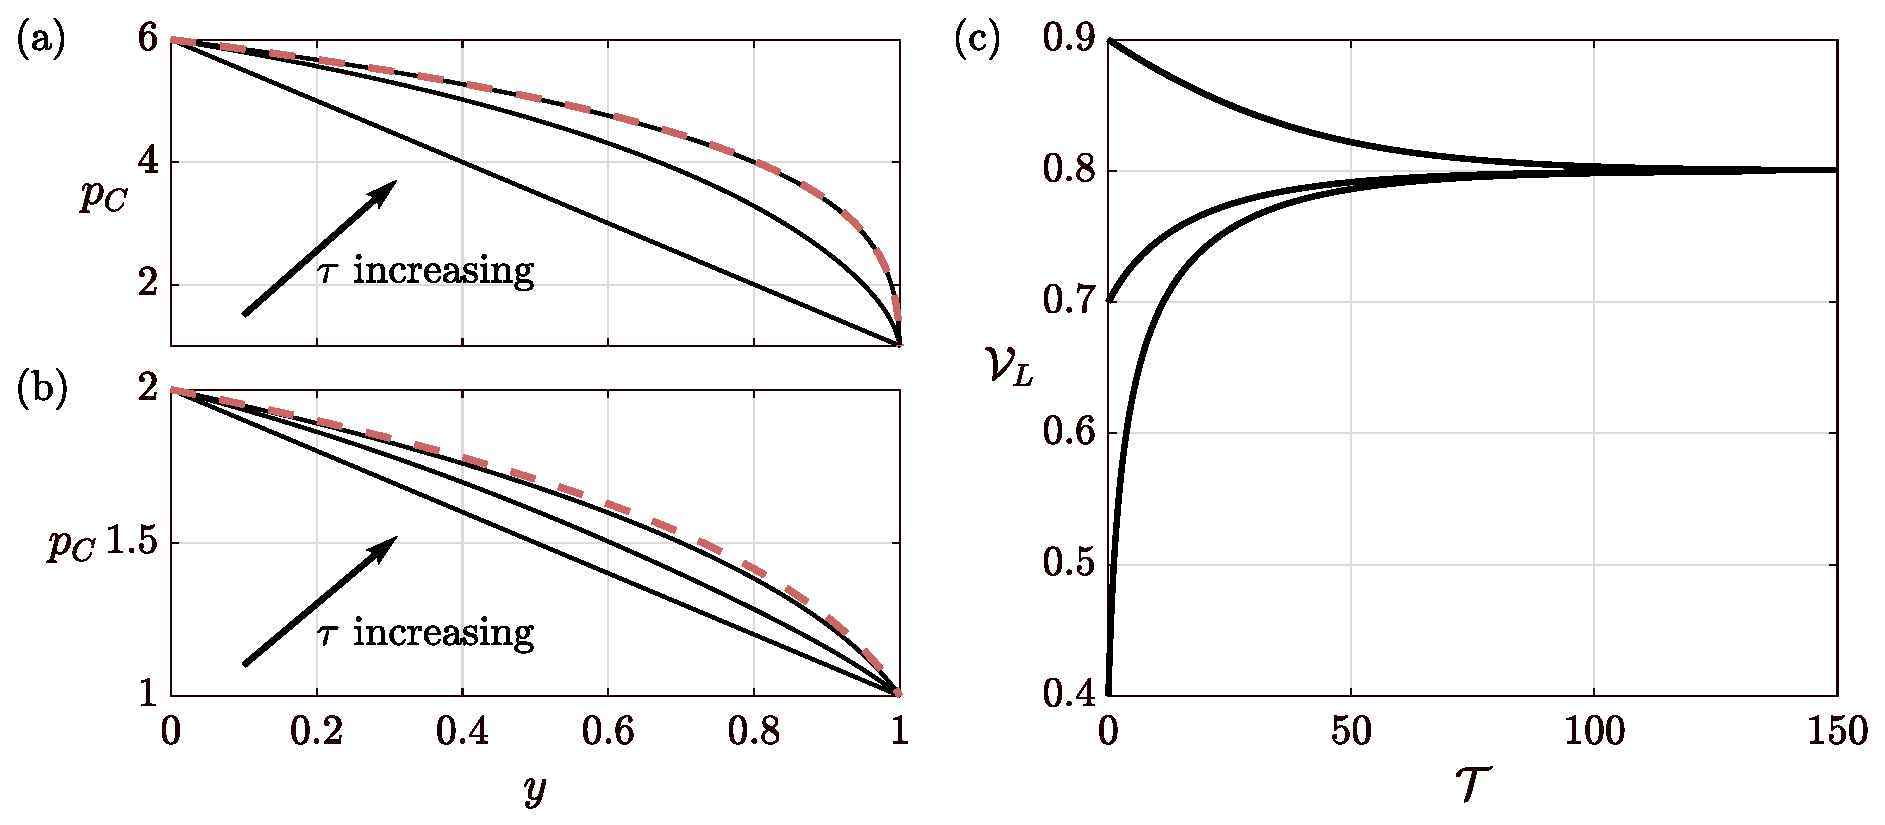
\includegraphics[width=1\linewidth]{Figures/Relaxation_Drainage}}  
  \caption{
  (a,b) Numerical solution of the conduit relaxation problem (\ref{eqn: pressure ODE})--(\ref{eqn: initial pressure}) for different boundary conditions (drop pressures), where the initial profile is a straight line.
  The dashed  line is the steady state solution given by  (\ref{eqn:  conduit  pressure}).
  In (a) $ \tau = 0, 0.01,0.03$, whereas in (b) $\tau =0,0.1,0.3$; with a larger pressure difference the steady state is reached much faster. 
  (c) The evolution of the left-hand drop volume given by  (\ref{eqn: volume ode}) \& (\ref{eqn: v initial}) for $ \mathcal{V} = 0.4,0.7 ,0.9$, in each case $ \alpha = 0.25$ and (\ref{eqn: V lim})  shows that the solutions tend to $0.8$.
  } \label{fig: drainage}
\end{figure}
%%%%%%%%%%%%%%%%%%%%%%%%%%%%%%%%% This was made with the matlab code:            Fig_Relaxation_Drainage.m
%%%%%%%%%%%%%%%%%%%%



As was detailed in \S \ref{sec: time scales}, the conduit relaxes on the  time scale  $t_{CL}  \sim \epsilon^{-4} $; this was derived from (\ref{eqn:  conduit  flux area}). 
Using (\ref{eqn:  conduit  flux area}), (\ref{eqn: area and flux})  and making the rescaling   $t = \epsilon^{-4}  \tau $  we derive an equation for the conduit pressure on the time scale of conduit relaxation: 
\begin{equation}
\pD{p_C}{{\tau}}{} = \frac{3}{70}\pD{}{{y}}{2}\left(p_C^4 \right)\quad \text{for $0<{y}<1$, $\tau >0$. } \label{eqn: pressure ODE}
\end{equation}
In    \S \ref{sec: junction} we deduced that the leading-order pressure in the junction regions is spatially uniform   and equal to the pressure in the  adjacent  drop and conduit   as long as $t\gg t_{J} \sim \epsilon $.
Since $t_{CL}\gg t_{J}$ as $\epsilon \to 0$,   the pressure at the ends of the  conduit  will be equal to the pressure in the corresponding drop,   so  the relevant boundary conditions for  (\ref{eqn: pressure ODE})   are given by 
\refstepcounter{equation} \label{eqn: pressure BCs}
\begin{equation}
p_C(0,\tau) = p_L(0), \quad p_C(1,\tau) = p_R(0) \quad   \text{for $\tau >0$  },  \tag{\theequation a,b}
\end{equation}
where the pressures in the left- and right-hand drops, $p_L$ and $p_R$, can be related to their respective volumes, $V_L $ and $V_R$, by   (\ref{eqn: drop height left}) and (\ref{eqn: drop height right}).
The problem is closed by prescribing an intial condition
\begin{equation}
    p_C( y,0) = \mathcal{P}(y)  \quad \text{for $0<y<1$.} \label{eqn: initial pressure}
\end{equation}
% \note{later}
% The solution of the resulting  boundary value problem  must be found numerically; we used  a central difference scheme for the spatial derivatives and the \textsc{Matlab} function   \emph{ODE15s} to find the time dependent  solution at each grid point.  
For a positive and sufficiently regular initial profile  we anticipate the long-time attractor to be the steady-state solution, so that 
\begin{equation}
p_C \to  p_{C \infty } = \left(  \left(p_R^4 -p_L^4  \right)y+p_L^4   \right)^{\frac{1}{4}} \quad \text{as $\tau \to \infty$.} \label{eqn:  conduit  pressure}
\end{equation}
Examples of the solution of the time dependent problem are shown in figures \ref{fig: drainage}a and b (solid lines), they 
 tend to  (\ref{eqn:  conduit  pressure}) (dashed line) as $\tau $ increases.
We are now in a position to describe the long-time behaviour of the system. 
% %%{f}igure %%%%%%%%%%%%%%%%%%%%%%
% \begin{figure} 
% \centering
%  {\includegraphics[height=0.45\linewidth]{Numerical_Height_Comparison}}  
%   \caption{A comparison of the composite solution with the numerical solution (dashed lines) at different times. 
%   The method for finding the composite solution is described in   \S \ref{sec: composite} although we have used (\ref{eqn: pressure ODE})  to find the height in the conduit as a function of time.} \label{fig: relax}
% \end{figure}
% %%%%%%%%%%%%%%%%%%%%%%%%%%%%%%%%% These were made with the matlab code:            Fig_Channel_relax.m
% %%%%%%%%%%%%%%%%%%%%


%  \note{quality control after} 
% \note{PLot are  and flux for comparison}
%     _______. _______   ______ .___________. __    ______   .__   __. 
%    /       ||   ____| /      ||           ||  |  /  __  \  |  \ |  | 
%   |   (----`|  |__   |  ,----'`---|  |----`|  | |  |  |  | |   \|  | 
%    \   \    |   __|  |  |         |  |     |  | |  |  |  | |  . `  | 
%.----)   |   |  |____ |  `----.    |  |     |  | |  `--'  | |  |\   | 
%|_______/    |_______| \______|    |__|     |__|  \______/  |__| \__/
\subsection{Droplet drainage} \label{sec: drainage}
On the time scale of drainage $t_{DD} \sim \epsilon^{-7} $, the pressure in the  conduit  is quasi-steady   and therefore given by the right-hand side of the equations in  (\ref{eqn:  conduit  pressure}).
We can then use (\ref{eqn: area and flux}b) to find that the flux in the conduit on this time scale is given by  
\begin{equation}
 Q  \sim  \epsilon^7 \frac{p_L^4-p_R^4}{35}. \label{eqn: flux}
\end{equation}
When $\epsilon \ll 1$   most of the fluid is contained in   the drops, with the  conduit  containing very little fluid.
So we can use   (\ref{eqn: flux odes}) to find ODEs for the volume in each drop.
Rescaling time with $t = \epsilon^{-7}  T$ and  substituting (\ref{eqn: flux}) into     (\ref{eqn: flux odes}a,b)  then gives
\refstepcounter{equation}\label{eqn: flux 1a} 
 \begin{equation}
 \pD{V_L}{T}{}= -\frac{p_L^4-p_R^4}{35}, \quad  \pD{V_R}{T}{}= \frac{p_L^4-p_R^4}{35}.  \tag{\theequation a,b} 
 \end{equation}
Since  the drop pressure is a linear function of the volume (see (\ref{eqn: drop height left}) and (\ref{eqn: drop height right})) we can define the constants  of proportionality in the left- and right-hand drops as
\refstepcounter{equation}\label{eqn: betas}
\begin{equation}
\beta_{L} = \frac{ Bo \, \besselj{0}{\Phi_{L} }}{\pi \alpha_{L}^2  \besselj{2}{\Phi_{L}}}  , \quad \beta_{R} = \frac{ Bo \, \besselj{0}{\Phi_{R} }}{\pi \alpha_{R}^2  \besselj{2}{\Phi_{R}}}  ,  \tag{\theequation a,b} 
\end{equation}
so that $p_L=\beta_L V_L$ and $p_R = \beta_R V_R$  and  (\ref{eqn: flux 1a}) can be written in terms of the drop volumes.
At leading order the total  volume $V$   is given by the sum of the volumes of the two drops, which is a constant since no fluid is leaving the system.
If  we then make the further scalings
\begin{equation*}
V_L = V \pazocal{V}_L, \quad V_R = V \pazocal{V}_R, \quad Q =  \frac { V^4  \beta_R^4 } { 35}  {\pazocal{Q}}  ,\quad T =   \frac{ 35} { V^3  \beta_R^4 }   {\pazocal{T}}    
\end{equation*}
 we  need only solve a single  ODE given by 
\begin{equation}
 \pD{\pazocal{V}_L}{\pazocal{T}}{} =-\alpha^4\pazocal{V}_L^4 + \left( 1-\pazocal{V}_L \right)^4, \label{eqn: volume ode}
\end{equation}
where   $\alpha^4 = \beta_L^4/ \beta_R^4  $. 
 Since we have chosen the left-hand drop to have  the largest   base radii we will have    $0< \alpha \leq1$.
 To close this problem we will need an initial volume for  the left drop 
 \begin{equation}
    \pazocal{V}_L(0) =   \mathcal{V}. \label{eqn: v initial}
 \end{equation}
The powers of four in  (\ref{eqn: volume ode}) suggest that there may be multiple steady-state solutions, but  it turns out that only one of them is real and in the range $[0,1]$, so the volume of the left drop can only tend to one value:  
\begin{equation}
\pazocal{V}_L \to \frac{1}{1+\alpha} \quad \text{ as } {\pazocal{T}} \to \infty. \label{eqn: V lim}
\end{equation}
Throughout we will refer to $\alpha $ as the positive real root of $\alpha^4$.
Equation  (\ref{eqn: volume ode}) is separable which allows us to easily find an   implicit solution.
Some examples of the evolution of the left-hand drop volume  are plotted in figure \ref{fig: drainage}c  for  different intial volumes, we have taken    $\alpha = 0.25$, so (\ref{eqn: V lim}) gives   $\pazocal{V}_L \to 0.8$.



% \begin{equation}
% \begin{aligned}
% \log\left(\frac{
% \left[\pazocal{V}_L-\frac{1}{1-\alpha}  \right]^{\frac{\left( 1-\alpha\right)^2}{4\alpha^3}} \left[\left(\pazocal{V}_L-\frac{2}{1+\alpha^2} \right) \pazocal{V}_L  + \frac{1}{1+\alpha^2} \right]^{\frac{1}{2\alpha^2}}  }{\left[\pazocal{V}_L-\frac{1}{1+\alpha}  \right]^{\frac{\left( 1+\alpha\right)^2}{4\alpha^3}}  }  \right) 
% \\+ \frac{\left( 1 -\alpha^2 \right)}{4\alpha^3 }\text{arg}\!\left(\frac{ -\alpha \pazocal{V}_L+\left(1-\pazocal{V}_L\right) i}{ 1-\pazocal{V}_L- \alpha \pazocal{V}_L i }  \right)  +C  = {\pazocal{T}}
% \end{aligned} \label{eqn: implicit volume}
% \end{equation} 
% % where $C $ is a constant of integration   found from the  initial conditions.
% While implicit and complicated in general, the solution can be written explicitly in the two limiting cases were either $\alpha^4\to 0$ (the left drop has a much larger base radius than the right) or $\alpha^4=1$ (the drops have the same base radius). In the case where $ \alpha^4 =1$ the volumes will tend to $1/2$ and the solution can be written explicitly as 
% \begin{equation}
% \pazocal{V}_L =\frac{1}{2} \left( 1 \pm  \frac{  1}{ \sqrt{A e^{ 2 {\pazocal{T}}} - 1}}\right), \quad A = 1+ \frac{1}{\left( 2\pazocal{V}_L(0)-1 \right)^2}. \label{eqn: V(tau)}
% \end{equation}
% where   the sign of the square root depends on the initial value, for $\pazocal{V}_L(0) >1/2$ we take the positive root ($\pazocal{V}_L$ decreases) otherwise we take the negative root. 
% When $\alpha^4=0$ 
% the solution to (\ref{eqn: volume ode}) is   given by 
% \begin{equation}
% \pazocal{V}_L=1- \left( 3 {\pazocal{T}} +\frac{1}{\left(1-\pazocal{V}_L(0)\right)^3} \right)^{-\frac{1}{3}}. \label{eqn: V alpha 0}
% \end{equation}
% Of course when $\alpha^4 = 0$ the right drop has a base radius of zero, so  it would not contain any fluid.  
% But, as we shall see later, as the base radius of the right drop is decreased, $\alpha$ rapidly tends to zero.

% While implicit and complicated in general, the solution can be written explicitly in the limiting case where  $\alpha^4=1$ (the drops have the same base radius). 
% In this case   the volumes will tend to $1/2$ and the solution can be written explicitly as 
% \begin{equation}
% \pazocal{V}_L =\frac{1}{2} \left( 1 \pm  \frac{  1}{ \sqrt{A e^{ 2 {\pazocal{T}}} - 1}}\right), \quad A = 1+ \frac{1}{\left( 2\pazocal{V}_L(0)-1 \right)^2}. \label{eqn: V(tau)}
% \end{equation}
% where   the sign of the square root depends on the initial value, for $\pazocal{V}_L(0) >1/2$ we take the positive root ($\pazocal{V}_L$ decreases) otherwise we take the negative root. 
 





% \note{all later or not at all}
%  Some examples of the drop inlet and outlet are shown in {f}igure \ref{fig: composite}  using the composite solution.
% The solid arrow indicates the direction of the flow; in general the height of  the interface decreases along the axis of symmetry where the fluid flows out of a drop and there is a local minimum near  where the fluid enters a drop.


% The location of the minimum is determined by the matching condition, with the solution in the junction decreasing  monotonically along the symmetry axis as the drop transitions to the conduit.
% It is then the outer solution in the  conduit  which determines whether the profile continues decreasing or whether there is a dip as shown in {f}igure \ref{fig: composite}b.
% The location of this dip will have some practical implications; the area of the  conduit  cross-section will be smallest here and so we expect the fluid velocity to be at its fastest.
% As is demonstrated in {f}igure \ref{fig: drainage}a the pressure gradient in the conduit near the inlet drop can become quite steep as the difference in drop pressures is increased. 
% Further, our piecewise composite solution will not have continuous derivatives where the conduit meets the drop, this explains the kink in the composite solution near $y=0$ as shown in {f}igure \ref{fig: composite}b. 









% using the above scalings the terms are balanced when $ t^* \sim \frac{3 \mu L}{ \delta^3 \epsilon^4 \gamma }$. 
% This is the relaxation time for $A$ and $ p_C$  and is much larger than the relaxation time scales we have seen so far. 
% Moreover, we can find the time scale for the equilibration of the pressure in the two drops ({\it {i.e.}\ignorespaces}  the time scale of drainage from one drop to the other).
% The terms in  (\ref{eqn: left drop vol}) are balanced when $ t^* \sim \frac{3 \mu L}{ \delta^3 \epsilon^7 \gamma }$. For the purposes of running an experiment this is the most relevant time scale since it gives an indication of how long the experiment can be run.
 















%     _______. _______   ______ .___________. __    ______   .__   __. 
%    /       ||   ____| /      ||           ||  |  /  __  \  |  \ |  | 
%   |   (----`|  |__   |  ,----'`---|  |----`|  | |  |  |  | |   \|  | 
%    \   \    |   __|  |  |         |  |     |  | |  |  |  | |  . `  | 
%.----)   |   |  |____ |  `----.    |  |     |  | |  `--'  | |  |\   | 
%|_______/    |_______| \______|    |__|     |__|  \______/  |__| \__/
 
\subsection{Composite solution} \label{sec: composite}
We are now in a position to construct an additive  composite solution for the film   height over the whole contact set  $ \Omega$. 
Since the solutions found in the drop and conduit regions are only valid in those regions we form a piecewise solution. 
In the left drop, $ y< 0$, the composite solution is found by adding the junction solution 
%(given by (\ref{eqn: junction leading order soln}) \& (\ref{eqn: junction height O(epsilon)})) 
to the drop solution 
%(given   by (\ref{eqn: drop height left})) 
and then subtracting the overlap, in this case  the two leading terms in the  limit  $\widebar{x}^2+\widebar{y}^2 \to \infty$ as shown in {f}igure \ref{fig: junction geometry}. 
The solution in the right drop is found in a similar way.
In the conduit, $0< y <1$,   we must find the junction solutions at either end of the conduit and add them both to the  conduit  solution (given by (\ref{eqn:  conduit  height}) \& (\ref{eqn:  conduit  pressure})), the overlaps are  then the   conduit solutions at $y=0 $ and at $y=1$, so these are both subtracted. 
An example of the composite solution is shown  in figure \ref{fig: composite}.
 %%figure %%%%%%%%%%%%%%%%%%%%%%
\begin{figure} 
\centering
 {\includegraphics[width=1\linewidth]{Figures/Composite_Solution_V2}}  
  \caption{
   The composite  solution  as described in \S \ref{sec: composite}.
      The dimensionless parameters used are $Bo = 20$,  $\alpha_L = 0.5$, $\alpha_R = 0.4$, $\epsilon = 0.05$, $V_L = 0.03$ and  $V_R = 0.03$.
      When the drops contain the same volume the drop with the smaller base radius has the higher pressure, so the flow is from left to right 
   } \label{fig: composite}
\end{figure}
%%%%%%%%%%%%%%%%%%%%%%%%%%%%%%%%% This was made with the matlab code:            Fig_Composite_Solution_V2.m
%%%%%%%%%%%%%%%%%%%%

 
%     _______. _______   ______ .___________. __    ______   .__   __. 
%    /       ||   ____| /      ||           ||  |  /  __  \  |  \ |  | 
%   |   (----`|  |__   |  ,----'`---|  |----`|  | |  |  |  | |   \|  | 
%    \   \    |   __|  |  |         |  |     |  | |  |  |  | |  . `  | 
%.----)   |   |  |____ |  `----.    |  |     |  | |  `--'  | |  |\   | 
%|_______/    |_______| \______|    |__|     |__|  \______/  |__| \__/
\subsection{Numerical validation} \label{sec: numerics}
% We proceed initially  by comparing the asymptotics with numerical simulation.
% We have found a number of solutions,  but before drawing   conclusions   we will compare with numerical simulation of the full problem.
% 
In this section we will numerically  solve  the full thin-film BVP given by  (\ref{eqn: lubrication}), (\ref{eqn: contact line})  and (\ref{eqn: initial}) on the domain   indicated in  {f}igure \ref{fig: geometry}f and compare the results with the asymptotic solutions we have obtained. 
The solution is  found  in \textsc{Comsol} Multiphysics\textregistered \  using the thin-film flow  toolbox.  
We specify the initial volumes of the two drops,  with this we can form a piecewise approximation to  the interface height and pressure using (\ref{eqn: drop height left}) and (\ref{eqn: drop height right})   in the drops and  (\ref{eqn:  conduit  height})     and   (\ref{eqn:  conduit  pressure}) in the conduit.
There will be discontinuities at either end of the conduit so we initially run the simulation on the junction relaxation time scale to smooth out the initial condition.
% \note{mention ladau levitch}

For intermediate values of $\epsilon$ ($\epsilon >\frac{1}{2}$) the numerical solution can be found in a matter of seconds, but as   anticipated,  on decreasing  $\epsilon$ we find run times increasing by multiple orders of magnitude,  with further implications for  computational time regarding    questions of microdevice design and fluid control. 
This underlines the utility of our asymptotic approach.
In figure \ref{fig: validation} we compare  various numerical solutions with our asymptotic predictions and show that as $\epsilon$ decreases  the solutions show excellent agreement.



  
In figure \ref{fig: validation} we compare the droplet drainage  solution  (see \S \ref{sec: drainage}) to   numerical solutions for various small  values of $\epsilon$.
In each simulation only the width of the  conduit  was altered  and the initial drop  volumes  were fixed.
 In figure \ref{fig: validation}a we see good agreement  over a range of values of $\epsilon$  for the volumes of the left (upper dashed line) and right (lower dashed line) drops  as a function of time.
The drainage solution can also be used to find the shear stress in the conduit.
In the $y$-direction the shear stress on the substrate is given by 
   \begin{equation}
{s} = \pD{v}{z}{} \bigg|_{z=0} =   -h  \pD{p}{y}{} = \frac{\left( \epsilon^2 - x^2\right) \left( p_L^4-p_R^4 \right) }{8 \sqrt{p_L^4 -\left(p_L^4 - p_R^4 \right)y   }}. \label{eqn: shear}
 \end{equation}
With this model the maximum shear stress is on $x=0$ at either $y=0$ or $y=1$ depending on the direction of the flow; the maximum will be at the junction of the  inlet drop.
In figure \ref{fig: validation}b we  compare the absolute  maximum   of the shear stress found in \textsc{Comsol}  with (\ref{eqn: shear}).
Again, as $\epsilon $ is decreased we see good agreement.
For the flux (given by (\ref{eqn: flux})),  we find  larger relative errors as can be seen in figure  \ref{fig: validation}c, especially on shorter time scales. 
Nevertheless there is still good agreement as $\epsilon$ is decreased.
This is shown  in figure    \ref{fig: validation}d, where the root mean squared error of the flux over a unit time interval  can be seen to decrease linearly  with $\epsilon$.


Finally, in {f}igure \ref{fig: validation 2}  we plot the composite  interface height (dashed line) along the centre of the  conduit, {\it {i.e.}\ignorespaces} on  $x=0 $ for different values of $\epsilon$.
The left and right panels show the profile in the respective drop regions and the central panels show the solution in the conduit region.
The solid line show the corresponding  numerical solution;
we see particularly good  agreement in the drop regions as $\epsilon $ is decreased.
In the conduit  the composite solution is able to pick out the location of the inlet dip (the flow is from left   to right), although it predicts a less sharp decrease in profile height.
This dip is  where the  maximum shear stress occurs in the numerical solution.




 
 
 %% Figure %%%%%%%%%%%%%%%%%%%%%%
\begin{figure} 
\centering
 {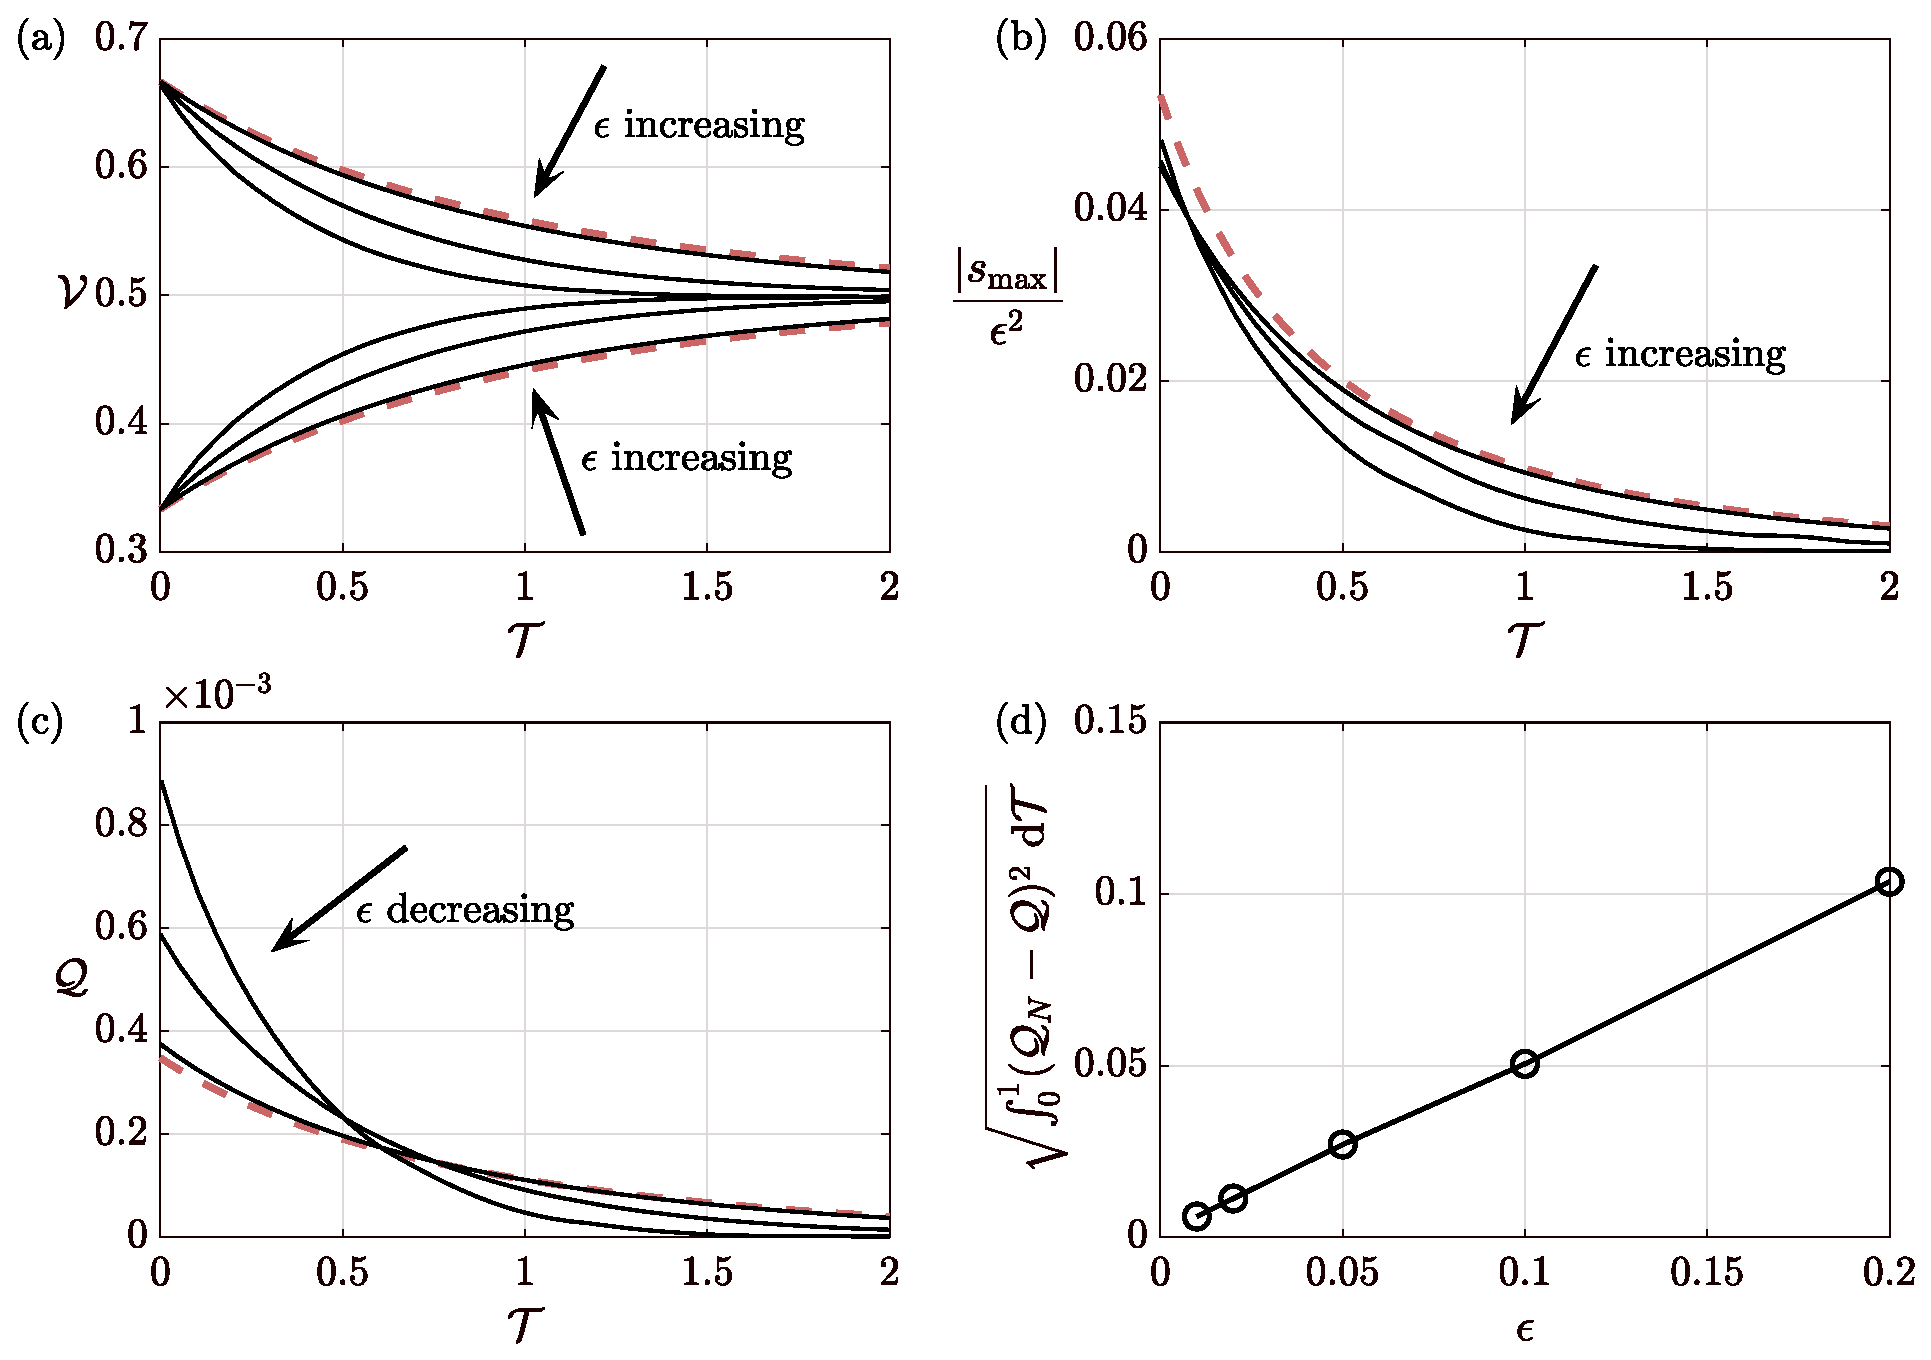
\includegraphics[width=1\linewidth]{Figures/Numerical_Validation_V2a.eps}}  
  \caption{
Comparison of \textsc{Comsol}    solutions with model predictions for different values of the small parameter $\epsilon$. 
In each case   the calculations were performed using  $\alpha_{L} = \alpha_{R} = 1$ and  $Bo=2$ with the intial volumes  $\pazocal{V}_L(0) = 2/3$  and    $\pazocal{V}_L(0) = 1/3$. 
(a)--(c) The solid lines show the numerical solution for   $\epsilon = 0.01,0.1,0.2 $  and the dashed line shows the  asymptotic approximation.
We compare  (a) the drop volumes,  given  (\ref{eqn: volume ode});   (b)  the maximum shear stress on the substrate, given by (\ref{eqn: shear}); and (c) the flux, given by (\ref{eqn: flux}).
(d) The root mean squared error of the flux over a unit time interval for different values of $\epsilon$, where $\pazocal{Q}_N$ is the numerical solution.
    } \label{fig: validation}
\end{figure}
%%%%%%%%%%%%%%%%%%%%%%%%%%%%%%%%% This was made with the matlab code:            Fig_Numerical_Validation_V2a.m
%%%%%%%%%%%%%%%%%%%%



 
%  For biological applications it is important to consider the shear stress induced by the flow, since this may  affect cell health (\cite{Varma2015AMicrofluidics.}) and development (\cite{Tsao2015FluidEnhancement}).
%  We define the dimensionless shear stress on the base of the  conduit  to be 

% %  \begin{equation}
% %  \tau^* =\mu_1 \pD{v^*}{z^*}{}  = \left( z^* -h^* \right) \pD{p^*}{y^*}{}.\label{eqn: shear dim}
% %  \end{equation}
% As $\epsilon \to 0$ we expect the shear stress to tend to the solutions   given by (\ref{eqn:  conduit  height}), (\ref{eqn:  conduit  pressure}) and (\ref{eqn: shear nondim}).
% In this case we can write it down explicitly as
% \begin{equation}
% {s} = \frac{\left( \epsilon^2 - x^2\right) \left( p_L^4-p_R^4 \right) }{8 \sqrt{p_L^4 -\left(p_L^4 - p_R^4 \right)y   }}, \label{eqn: shear}
% \end{equation}
% if the initial volumes of the drops are known we can  use (\ref{eqn: drop height left}b), (\ref{eqn: drop height right}b)  and the solution of (\ref{eqn: volume ode})   in (\ref{eqn: shear}) to estimate the shear stress on the substrate as a function of time.




 %% Figure %%%%%%%%%%%%%%%%%%%%%%
\begin{figure} 
\centering
 {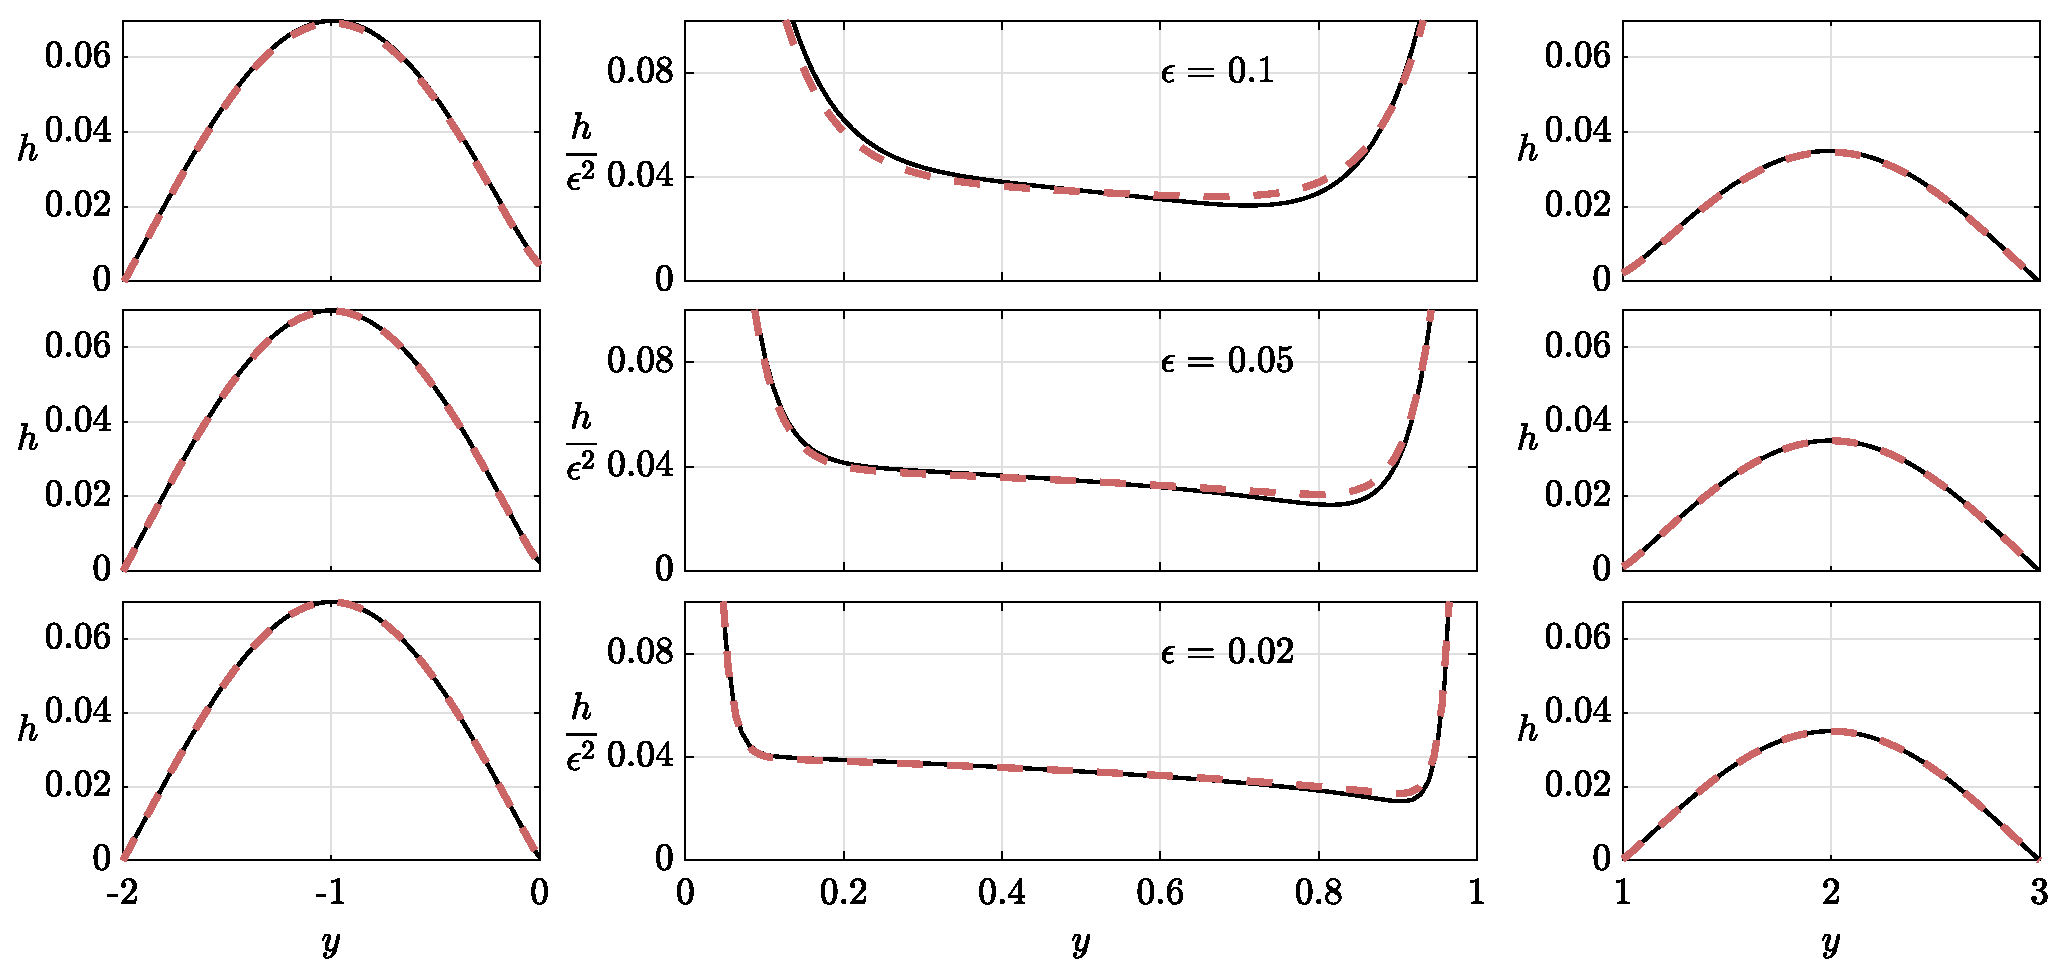
\includegraphics[width=1\linewidth]{Figures/Numerical_Validation_V2b.eps}}  
  \caption{
Comparison of \textsc{Comsol}    solution  with the composite solution described  in  \S \ref{sec: composite} on $x=0$.
The calculations were performed using  $\alpha_{L} = \alpha_{R} = 1$ and  $Bo=4$ with the intial volumes  $\pazocal{V}_L(0) = 2/3$  and    $\pazocal{V}_L(0) = 1/3$. 
The solid lines show the numerical solutions     and the dashed lines   the corresponding   asymptotic approximation. 
    } \label{fig: validation 2}
\end{figure}
%%%%%%%%%%%%%%%%%%%%%%%%%%%%%%%%% This was made with the matlab code:            Fig_Numerical_Validation_V2a.m
%%%%%%%%%%%%%%%%%%%%







\subsection{Physical and mathematical constraints}
\label{sec: constraints}

 The presence of Bessel functions in the drop solution (\ref{eqn: drop height left})  immediately suggests a regime outside the applicability  of our analysis; we cannot allow the height or volume  to be negative and since the pressure is proportional to the volume we also require the pressure to be positive.
 If we denote by  $  j_{0,0}$   the smallest positive root of $ \besselj{0}{x}=0$, then the pressure is positive as long as  $ \Phi_L^2<j^2_{0,0} \approx 5.78$. 
 This puts an upper limit on the possible base radii used.
 For the parameters given in table \ref{tab: parameters}, a drop with a base radius greater than \SI{5.2}{\milli \metre} is    beyond the scope of this  analysis.
 Although, if we were to flip the device upside down (or equivalently use a less dense covering fluid), so that gravity acted in the opposite direction, the Bessel functions would be replaced with modified Bessel functions.
 The modified Bessel functions do not oscillate and so there would be no upper limit on the size of the base of the drops.


 An important feature of these devices are  the large advancing and small receeding  contact angles, $\theta_A$  and $\theta_R$ respectively, which  allows the volume of fluid  in a drop to change significantly without the contact line moving.
 \cite{Walsh2017MicrofluidicsWalls} observe values of  $\theta_R \sim \SI{3}{\degree}$ and $ \theta_A\sim \SI{70}{\degree}$.
 Using the leading order solutions (\ref{eqn: drop height right}), (\ref{eqn: drop height left}) and    (\ref{eqn:  conduit  height}), we define the contact angles in the left- and right-hand  drops and  the conduit, denoted by  $\theta_L $, $\theta_R $ and $\theta_C$ respectively, to be 
 \refstepcounter{equation}   \label{eqn: angles}
 \begin{equation}
       \theta_L = \frac{\delta  \alpha_L}{ \kappa\!\left( \Phi_L\right)}  p_L,\quad      \theta_R = \frac{\delta  \alpha_R}{ \kappa\!\left( \Phi_R\right)}  p_R,\quad    \theta_C = \delta \epsilon \, p_C, \quad      \kappa\!\left( \Phi\right) =\frac{ \Phi  \besselj{0}{\Phi }}{\besselj{1}{\Phi }   } .   \tag{\theequation a--d}
\end{equation} 
The advancing contact angle will not be exceeded in the drop or conduit regions without violating our intial thin-film assumption that $\delta \ll 1$.
The same however cannot be said of the junction regions; as can be seen in    figure \ref{fig: junctions} there are  singularities  in the second-order solution  at the points  $(\widebar{x},\widebar{y}) = (\pm 1,0)$.
In practise  the contact line near this corner will  move outwards until the contact angle falls to the advancing angle.
We expect the smoothing of the corner to happen on the length scale of the junction region ({\it {i.e.}\ignorespaces} the width of the conduit).
In the thin-film regime it is the receding angle that is likely to be of more significance.
Without loss of generality  we assume that the left-hand drop has the lower pressure.
Then, on the time scale  $t \gg t_{CL} \sim \epsilon^{-4}$, the   smallest    contact angle  in the conduit  will occur at $y=0$,  where  $p_L = p_C$.
We can then combine   (\ref{eqn: angles}a) and  (\ref{eqn: angles}b)  to give
\begin{equation}
    \theta_C = \frac{\epsilon}{\alpha_L}   \kappa\!\left( \Phi_L\right)  \theta_L.
\end{equation}
Since we have imposed an upper limit on $\Phi_L$, we find that  the function  $\kappa$ only has values in the range $[ 0,2]$.
We then  deduce that the contact angle in the conduit is always less than in the drops as long as  $ \epsilon/\alpha_L <1/2   $ ({\it {i.e.}\ignorespaces} $2 a< R_L$),  with a similar result if the right-hand drop has the lower pressure.
Combining (\ref{eqn: angles}c) with the expression for the pressure as a function of volume in the left-hand drop (see (\ref{eqn: drop height left}) \&  (\ref{eqn: betas})) the minimum leading-order contact angle is given by 
\begin{equation}
\theta_{\text{min}} =  \delta \epsilon \beta_L  V_L. 
\end{equation}
Again we find  a  similar result when the right-hand drop has the lower pressure.
So, as long as $\theta_{\text{min}} > \theta_R \sim 0.05 $, the contact line will remain pinned (other than in the junction region where, as mentioned above, the corners will be smoothed out).


 

 \subsection{A survey of fluxes and shear stresses} 
 \label{sec: trends}
 
 

%%%%%%%%%%%%%%%%%%%%%%%%%%%%%%%%%%%%%%%% FIGURE %%%%%%%%%%%%%%%%%%%%%%
\begin{figure} 
\centering
 {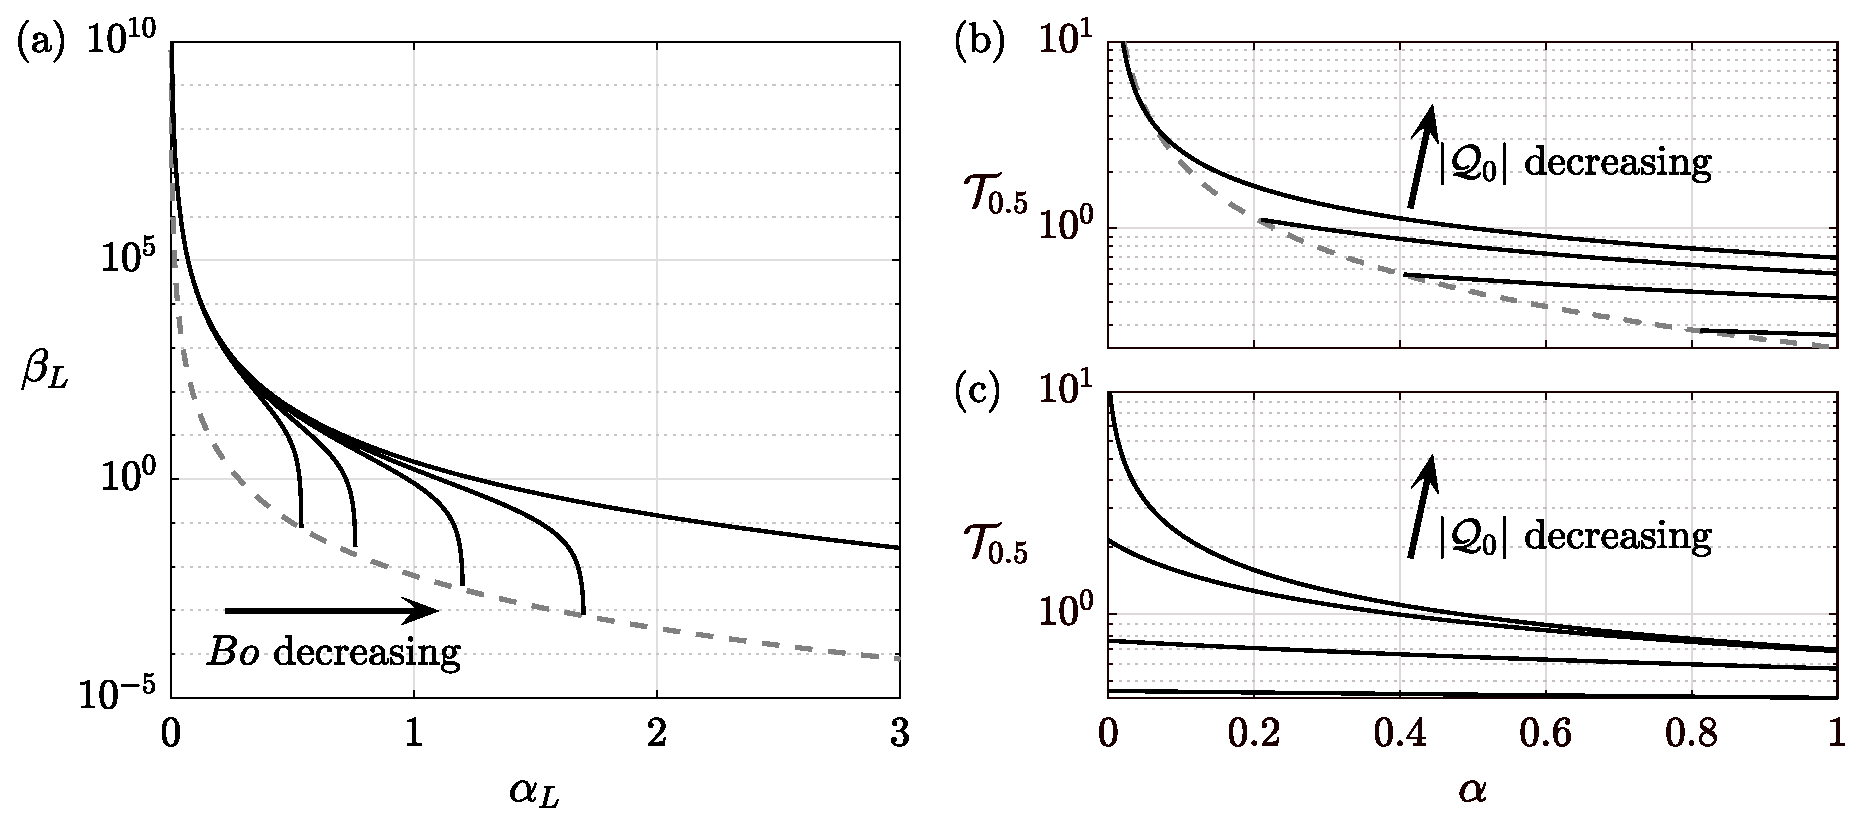
\includegraphics[width=1\linewidth]{Figures/Parameters_V2}}  
  \caption{ 
(a) A plot of $  \beta_L   $    for $Bo = 0.1, 2, 4, 10, 20$, where $\beta_L$ is the ratio of the dimensionless  drop pressure to volume for the left-hand drop  given by (\ref{eqn: betas}). 
The dashed line shows the boundary on  which  $\sqrt{Bo}\, \alpha_L = j_{0,0} $. 
  (b,c) The time taken for an initial flux $\pazocal{Q}_0$  to reduce by $50\%  $  as a function of $\alpha$. In (b) the intial flow is from left to right $\pazocal{Q}_0 = 0.01, 0.2, 0.4, 0.8$  and in (c) the intial flow is from right to left $\pazocal{Q}_0 =  -0.4, -0.2,  -0.05, -0.005$.
  } \label{fig: alpha beta}
\end{figure}
%%%%%%%%%%%%%%%%%%%%%%%%%%%%%%%%%%%%%%%%%%%%%%%%%%%%%%%%%%%%%%%%%%%%%%%%%
% This was made with the matlab code:            Fig_Parameters_V2.m        
%%%%%%%%%%%%%%%%%%%%%%%%%%%%%%%%%%%%%%%%%%%%%%%%%%%%%%%%%%%%%%%%%%%%%%%%%



We have already identified one way in which the footprint of the device   can significantly alter the  time scales involved.
In \S \ref{sec: times}  we showed that   the time scale of drop drainage scales with $\epsilon^{-7}$, where $\epsilon = a/L$.
Three further parameters that affect the behaviour on this time scale are $\alpha$, $\beta_L$ and $\beta_R$.
In figure \ref{fig: alpha beta}a we plot $\beta_L$ (a plot of $\beta_R$ would look very similar),  a log scale has been used to highlight that it  varies  over several orders of magnitude.
Recall that $\beta_L$ is the ratio of pressure to volume in the left-hand drop.
Varying the Bond number does not have much influence on $\beta_L$ suggesting that gravity is not having a large impact on the pressure in a   drop at leading order.
In contrast shrinking the  size of the base radius of the drop  $\alpha_L$  massively increases the pressure for a given volume.
The ratio of $\beta_L $ and $\beta_R$ is defined as  $\alpha$, which inter-alia  determines     how much fluid we would expect in each drop at equilibrium (see (\ref{eqn: V lim})).
As the relative sizes of the drop base radii become more disparate $\alpha$ quickly decreases (since we have assumed the left-hand drop has the larger base radius) and $\pazocal{V}_L \to 1$. 

One of our main interests is in determining the conditions for an approximately constant  flux in the conduit. 
We  initially look for fluxes that decrease by  $X \%$ and determine how long this takes. 
On the time scale of drainage we approximate the initial flux  $ \pazocal{Q}_0$  using the right-hand side of  (\ref{eqn: volume ode}),  figure \ref{fig: alpha beta}c and d shows   the time taken $\pazocal{T}_{0.5}$ for the   initial flux   to reduce by $50\%$ for a given value of $\alpha$.  
Since we assumed that the $0 <\alpha \leq1$ changing the sign of the flux gives different results.
Positive fluxes are shown in  figure \ref{fig: alpha beta}c, the second term in the right-hand side of \ref{eqn: volume ode} is always negative, as $\alpha \to 0$ there will be fewer  positive solutions, this is indicated by the dashed line in  figure \ref{fig: alpha beta}c. 
With negative fluxes the trend is similar but there is no bound on the possible fluxes as shown in  figure \ref{fig: alpha beta}d.  
This shows that maintaining an approximately constant  flux over long time periods requires  very  small fluxes, although in practice such small fluxes may not be desired.


The numerical solution of  (\ref{eqn: lubrication}), (\ref{eqn: contact line})  and (\ref{eqn: initial})   has shown that the maximum shear stress occurs where the  conduit  has the smallest cross-section, the dip near the inlet drop.
As $\epsilon \to0$ this dip moves closer to the drop as can be seen in  {f}igure \ref{fig: validation}a.
In general the shear stress quickly decreases as we move away from the maximum due to the   $ 1/\sqrt{y}$ dependence in (\ref{eqn: shear}), so avoiding the highest shear stresses can be achieved by avoiding the region  near the inlet drop. 
 \cite{Walsh2017MicrofluidicsWalls} show that human embryonic kidney (HEK)   cells can grow normally in their devices, although they were not concerned with the shear stress in this case.
 \cite{Stathopoulos1985ShearVitro} state that  a shear stress greater than \SI{2.6}{\newton \per \meter^2} has a significant affect on the  viability of HEK cells.
Since the  shear stress scales with $  \epsilon^2$, a narrow  or long  conduit  will be required to keep it to an acceptable level. 
Although, as shown in {f}igure \ref{fig: circuits}, in the thin-film limit the shear stress will typically be less than this.
A large shear stress is associated with a large flux, which means  higher shear stresses if they do occur would be short lived.


 
 A selection of solutions to the leading-order drainage time problem (\ref{eqn: volume ode}) are shown in {f}igure \ref{fig: circuits}, where the flux and shear stress are given by (\ref{eqn: flux}) and (\ref{eqn: shear}). 
 Starting with two drops each of base radius \SI{3.2}{\milli \meter} connected by a  conduit  of length \SI{10}{\milli \meter} and width \SI{1.2}{\milli \meter} and initial volumes of \SI{18}{\micro \litre}  in the left drop and \SI{12}{\micro \litre}  in the right, we show how the flow rate and maximum shear stress change with the  base radii of the  right-hand drops, the  conduit  width and length and the intial volumes of the  right-hand drop.
 As we alluded to earlier,  the pressure in a drop is very sensitive to the radius of the base,  figure \ref{fig: circuits}a  shows that changing the base radius of the right-hand drop by  \SI{0.4}{\milli \meter} completely changes the direction of flow.
 In figures  \ref{fig: circuits}b and c we are   changing the value of $ \epsilon $  and as such the variation in the solution is over a much longer time scale.
 
  


 %%{f}igure %%%%%%%%%%%%%%%%%%%%%%
\begin{figure} 
  \centering{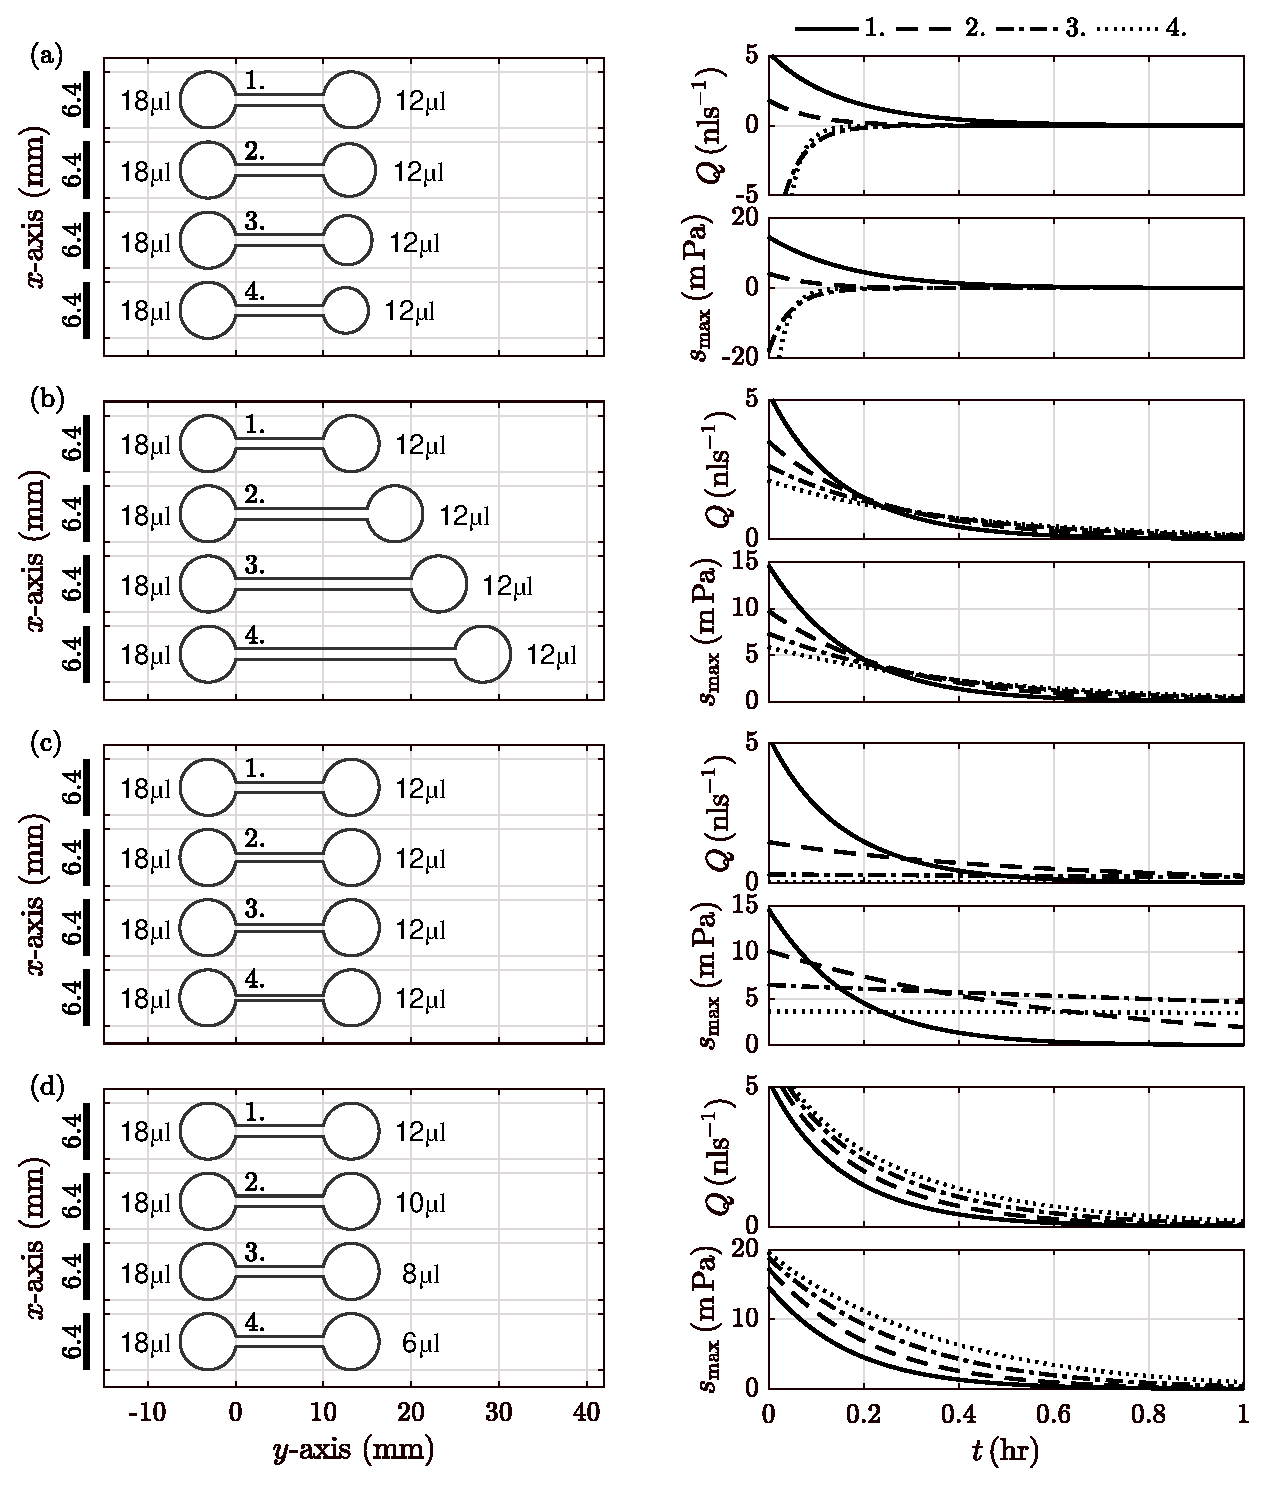
\includegraphics[width=1\linewidth]{Figures/Circuits_V2.eps}} 
    \caption{
    There are six dimensional parameters that can be  modified to get a desired flow rate or maximum shear stress.
    In these figures we modify (a)  the base radius of the right drop;  (b) the length of the conduit; (c) the width of he conduit; and (d) the volume of the right-hand drop. 
    The geometries and volumes represent typical values that are within the limits of the thin-film model with  a time scale of minutes to  hours.
    As can be seen in all plots this results in quite small fluxes and correspondingly small shear stresses.
    }  \label{fig: circuits}
\end{figure}
%%%%%%%%%%%%%%%%%%%%%%%%%%%%%%%%% This was made with the matlab code:                               Fig_Flux_Shear_Circuits_V2.m
%%%%%%%%%%%%%%%%%%%%
 




 
 
 



% For instance if we wanted a flux of $ \SI{50}{\nano \litre \per \second}$ to reduce by less than $10\%$ over $\SI{5}{\hour}$ we could take $\alpha_L = 0.31$, $\alpha_R = 0.3$, $L = \SI{10}{\milli \metre}$, $ a = \SI{1}{\milli \metre}$, $v^*_L = \SI{0.7}{\micro \litre}$ and $v^*_R = \SI{0.3}{\micro \litre}$.
% \note{Find multiple solutions for same initial flux and plot them all?}

   
as alpha get small right-hand side of ODE shows that flux is negative hence the dashed line in figure \ref{fig: alpha beta}b there are not positive fluxes which satisfy this 

 
 \section{Model extensions} \label{sec: extensions}

 
 
 \subsection{Passive networks} \label{sec: networks}
 
%  \note{how should this be non-dimensionalised?}
 In the introduction we  stated that one of the advantages of the new kind of microfluidic devices described here is that complex patterns of drops and conduits can be easily printed.
Now we show how the simple model derived above can similarly  be extended to arbitrary networks of drops and conduits.
To   be able to form networks we introduce ``nodes", these are the junctions formed where two or more conduits intersect. 
 They will be essential in constructing more complex networks and we will show that they are easily accounted for in the leading order model.
 There are three possible ways in which a simple  circuit could be extended that are consistent with our analysis (i) a new  conduit  could be connected to an  existing one via a node, the other end of which is connected to  drop or node; (ii)  a new  conduit  could be connected to an  existing drop, the other end of which is connected to  drop or node; (iii) two existing drops or nodes could be connected by a new conduit.
  As with the junction region connecting a  conduit  to a drop we could use a Schwarz-Christoffel to transform a node connecting multiple conduits   to a simpler domain and find the transformation interface shape in this region.
Instead we use  an  analogy  with electric circuits.
 %% Figure %%%%%%%%%%%%%%%%%%%%%%
\begin{figure} 
\centering
 {\includegraphics[width=0.8\linewidth]{Figures/Network_Nodes_V2.eps}}  
  \caption{  
  For a given drop the change in volume depends on the flux in all connected conduits.
  Similarly the pressure in node depends on the fluxes of all connected conduits.
  In each case the other end of the  conduit may be connected  to either a drop or a node. 
    } \label{fig: Network problem}
\end{figure}
%%%%%%%%%%%%%%%%%%%%%%%%%%%%%%%%% This was made with the latex code: Network_Nodes.m
%%%%%%%%%%%%%%%%%%%%

 The flow of fluid in networks of pipes  has been modelled 
 by making an analogy with Kirchoff's  laws for the current and voltage in an electrical circuit, for instance see  \cite{WilliJagerBenSchweizerViscousPipes} and 
 \cite{Marusic-Paloka2001FluidPipes}.
 These laws  tell us that the total fluid flowing into a node is equal to the total amount of fluid flowing out,  {\it {i.e.}\ignorespaces} mass is conserved at each node.
The volume of a drop now depends on the flux in each connected conduit as  shown in  figure  \ref{fig: Network problem}.
For a network consisting of $n$ drops and $m$ nodes we have $n$ time dependent  ODEs  describing the drop volume and $m$ algebraic equations for conservation of mass in each node. 
The drops are labelled with    $1, \dots, n$ and the nodes  with $ n+1, \dots, n+m$, we define $ \Pi_i$ to be the set of objects (drops or nodes) connected to object $i$.
The initial volumes in the drops are assumed to be known and thus the initial pressures in each drop  are found with the function 
\begin{equation}
    f\!(v;R)  =  \frac{B\, \gamma\,  \besselj{0}{\sqrt{B}\, R }  }{\pi R^2  \besselj{2}{\sqrt{B}\, R } } v , \quad B = \frac{\Delta \rho\, g}{\gamma} .
\end{equation}
Note that this is the general dimensional version of (\ref{eqn: betas}).
Generalising the equation for the flux into a drop connected to a single conduit gives
\begin{equation} 
     \pD{V_N}{t}{}  = \sum_{i\in\Pi_N} Q_{N,i},\quad Q_{N,i} = -\frac{a_{N,i}^7}{105 \gamma^3 \mu_1 L_{N,i}}\left( p_N^4 -  p_{i}^4  \right), \quad   p_N =  f( v_N; R_N).
\end{equation}
And by analogy with Kirchhoff's laws, in the nodes we have 
\begin{equation} 
     \sum_{i\in\Pi_K} Q_{K,i}=0, \quad Q_{K,i} = -\frac{a_{K,i}^7}{105 \gamma^3 \mu_1 L_{K,i}}\left( p_K^4 -  p_{i}^4  \right).
\end{equation}
The initial pressures in the nodes are unknown, so we must first solve an  algebraic system  of equations to find the initial values before using an ODE solver.
 Using this theory we have developed a GUI which allows arbitrary networks to be drawn and the resulting ODEs solved. 
 An example of GUI is shown in figure \ref{fig: GUI}, complex networks can be defined in a matter of seconds and the resulting ODEs rapidly solved.
%%%%%%%%%%%%%%%%%%%%%%%%%%%%%%%%%%%%%%%% FIGURE %%%%%%%%%%%%%%%%%%%%%%
\begin{figure} 
\centering
 {\includegraphics[width=1\linewidth]{Figures/GUI_example2.png}}  
  \caption{ 
  Combining the  network problem described in \S \ref{sec: networks} with a tool for drawing arbitrary    networks, this   will hopefully provide a way to rapidly test potential experimental setups.
  }   \label{fig: GUI}
\end{figure}
%%%%%%%%%%%%%%%%%%%%%%%%%%%%%%%%%%%%%%%%%%%%%%%%%%%%%%%%%%%%%%%%%%%%%%%%%
 %%%%%%%%%%%%%%%%%%%%%%%%%%%%%%%%%%%%%%%%%%%%%%%%%%%%%%%%%%%%%%%%%%%%%%%%%


\subsection{Active pumping}
As we noted in the introduction, passive pumping is not the only mechanism by which a flow can be maintained in the conduit.
Adapting the existing model to allow for fluid to be fluid   pumped directly into (or out of) the conduit either with a drop at one end or pumps at both  means that the boundary conditions in the conduit need to be changed.
We assume that on the time scale of drainage  the flux in the conduit is equal to the flow rate of the pump, if there are pumps at both ends they are  assumed to pump fluid into an out of the conduit at the same rate.
 Then the left-hand side of (\ref{eqn: area and flux})b is known and we only need a single boundary condition to solve the ODE, when the conduit is connected to a drop we fix the pressure at that end, otherwise we need to know the initial volume of the conduit which fixes the interface height. 




%     _______. _______   ______ .___________. __    ______   .__   __. 
%    /       ||   ____| /      ||           ||  |  /  __  \  |  \ |  | 
%   |   (----`|  |__   |  ,----'`---|  |----`|  | |  |  |  | |   \|  | 
%    \   \    |   __|  |  |         |  |     |  | |  |  |  | |  . `  | 
%.----)   |   |  |____ |  `----.    |  |     |  | |  `--'  | |  |\   | 
%|_______/    |_______| \______|    |__|     |__|  \______/  |__| \__/

\section{Discussion} \label{sec: discussion}

Using the standard thin-film equation and the novel geometry of the device    we have developed   an asymptotic model  for  the flux in the  conduit   and the  volumes of the connected drops, together with a composite solution for the interface  height,  taking account of the junction regions.
On the drainage time scale we found an analytic  solution, which shows good agreement with numerics when the aspect ratio of the  conduit  is small, {\it {i.e.}\ignorespaces} $\epsilon \ll1$ (see {f}igure \ref{fig: validation}). 
When designing an experiment with a  dumbbell configuration  there are six dimensional parameters that can be  modified ($a$, $L$, $\alpha_L$, $\alpha_R$, $v_L$ and $v_R$); the width and length of the channel, the base radii of the two drops as well as the initial volume of fluid contained in each.
 Given a required flow rate, drainage time, shear stress (or other property)  there is clearly a large solution space in which to  search to find a circuit with the desired properties.
 Such an inverse problem is beyond the scope of the current paper, but  the effect of modifying each of these parameters in turn on the leading order drainage time solutions is easily determined as shown in {f}igure \ref{fig: circuits}.
%  In general, if a solution exists satisfying a single criteria (e.g.  a quasi-steady flux), there will be multiple solutions.

 We have shown that maintaining an approximately constant    flux may not be straightforward if larger fluxes are needed for longer time scales.
Nonetheless  the more extreme geometries will be the most appropriate and also the most amenable to our analysis.
The time scale of drainage has been shown to be ultra sensitive to the aspect ratio of the conduit  and  thus it is the geometry that is the most important factor in achieving an approximately constant   flux.
However,  the  height of the  conduit  is not constant, so the flow in different regions of the  conduit  will be different.
If one requires near constant fluid velocities in different regions of the  conduit  such extreme geometries will not be appropriate.
Thus if both constant temporal and spatial flow is desired there is ultimately a trade-off  between the two, though spatial variation is much less sensitive.
In addition to these considerations low stresses will often be required for cell handling experiments.
There will be a maximum in the shear where the fluid flows into a drop,  occurring in the dip identified earlier.
This can be easily avoided given how quickly the shear stress decreases as we move away from this region. 
For much longer running experiments, there are several choices available to extend the  time over which the flux is approximately constant.
The first and most obvious is to use larger volumes of fluid.
In future  work 
we  will  extend the simple dumbbell model by considering what happens when the vertical length scale is comparable to the horizontal ones; in this case  the pressure no longer depends linearly on the volume and far more complex flow patterns emerge. 
% Secondly networks of drops and conduits may allow more complex  flow patterns  maintaining an approximately constant  flux in a particular conduit.
% The simplicity of the model presented here means that we can easily extend it to allow for much more complicated geometries involving multiple drops connected by multiple conduits.
% By analogy with the Kirchhoff laws we will be able to find a closed system of ODEs describing arbitrary networks.
% Finally we could print only a  conduit   and   pump fluid directly through it.
% Analysing this generalisation can also be explored with   the current framework requiring little modification. 


In summary, we have  found  an asymptotic model describing the flow   between two fluid drops connected by a long, thin rivulet.
The model compares favourably with  numerical solution as the small parameter $\epsilon$ is decreased, and finds application to wall-free microfluidic circuits.
% The model will simplicity of the model will allow for experimental design  


% We will then be in a position to compare this model to experimental data.
 



 




 


% %%%%%%%%%%%%%%%%%%%%%%%%%%%%%%%%%%%%%%%% FIGURE %%%%%%%%%%%%%%%%%%%%%%
% \begin{figure} 
% \centering
%  {\includegraphics[width=1\linewidth]{Figures/GUI_example1.png}}  
%   \caption{ 
%   }  
% \end{figure}
% %%%%%%%%%%%%%%%%%%%%%%%%%%%%%%%%%%%%%%%%%%%%%%%%%%%%%%%%%%%%%%%%%%%%%%%%%
%  %%%%%%%%%%%%%%%%%%%%%%%%%%%%%%%%%%%%%%%%%%%%%%%%%%%%%%%%%%%%%%%%%%%%%%%%%






 

 

\bibliographystyle{jfm} 
\bibliography{Mendeley}

\end{document}
